\chapter{动态采用检查点备份技术的\\GPU主动抢占策略}
\label{chap:PEP}

本章针对堆叠异构系统的多任务切换的高上下文开销问题,提出了动态采用检查点备份技术的GPU主动抢占策略。
\ref{sec:pepintroduction}节概述了本章的研究。
\ref{sec:pepbackground}节和 \ref{sec:pepmotivation}节介绍了本章主动抢占策略的研究背景和动机。
\ref{sec:peprelated}节则介绍了与本章相关的先前工作,比较了这些工作和本章工作的不同。
\ref{sec:pepdesign}节和~\ref{sec:pepexperiment}节分别介绍了本章的GPU主动抢占策略和实验结果。
最后,\ref{sec:pepconclusion}节总结了本章的工作。




\section{研究概述}
\label{sec:pepintroduction}

GPU由于其大规模并行处理能力,已经在高性能计算,机器学习和科学计算等领域得到广泛应用~\upcite{anderson2008general,mosegaard2005real,parker2010optix,podlozhnyuk2007black,tensorflow,ec2}。
这些领域的计算如今以服务的形式存在于数据中心或云上,而GPU则可作为基础硬件资源提供给不同的用户。
多任务处理在GPU中为支持并行服务和任务已经变得必不可少。
已经有些重要的硬件特性支持多任务处理,例如NVIDIA Kepler体系结构提供的HYPER-Q~\upcite{kepler}、AMD支持的命令处理机制等~\upcite{mantor2012amd,rogers2013heterogeneous,amdr9}。
虽然已经有这些机制支持多任务处理,但还需要更多的工作来支持真正的多任务处理机制~\upcite{adriaens2012case,calhoun2012preemption}。

上下文切换是一种在CPU中常用的支持并行性的技术~\upcite{li2007quantifying},如今该技术已经被应用到了GPU以支持多任务切换~\upcite{adriaens2012case,pai2013improving}。
CPU的进程相对来说非常轻量化,所以在上下文切换和时分任务等应用上非常快速高效。
但是,一个CUDA线程的上下文相比于CPU的线程却是非常大的~\upcite{nvidia2011nvidia}。
比如在NVIDIA GTX 980 GPU上~\upcite{nvidia980s},上下文包括每个流多核处理器的256KB的寄存器和96KB的共享内存。
对于一个含16个流多核处理器的GPU,其上下文大小达到了5664KB。
存储这样大的上下文需要耗费大量的存储带宽,并带来严重的性能损失~\upcite{chen2017effisha,lin2016enabling}。

之前已经有许多工作探索降低GPU上下文切换开销的方法。
最早出现的技术是让上下文切换仅在一部分流处理器核上进行,这样其他的流水里器核就能保持继续执行~\upcite{tanasic2014enabling}。
被切换的流处理器核会完全停止执行指令,以完成上下文的存取。
这些操作对于存储带宽的要求依然非常高。
之后出现一种方法,让一部分线程块继续执行直到完成,而只切换一部分线程块的上下文~\upcite{wang2016simultaneous}。
这样可以最大化的利用程序访存和上下文访存的重叠并行性。
这个技术被进一步加强扩展,允许在需要抢占时每一个流处理器核内部的不同线程块同时进行排空执行(直至线程块完成)、丢弃(满足幂等性)、和上下文切换~\upcite{park2015chimera}。
这些选择均取决于每个线程块对于抢占的终止时间的要求。
除了这些工作,一种轻量级的上下文切换技术被设计来降低需要保存在片外存储器的上下文大小~\upcite{lin2016enabling}。
所有这些方法都是通过被动的方法来实现抢占,即只有当抢占请求到来以后才激活所有的操作。
因此,如果没有丢弃操作,抢占延迟依然是对性能的一大挑战。

本章提出了一种动态主动的抢占机制,称为PEP。
这种抢占机制能够显著降低抢占延迟和开销。
通过观察内核函数从CPU到GPU的启动过程,我们发现内核函数的实际执行总是在内核函数启动之后。
从一个内核函数在CPU启动到开始在GPU执行,大约需要几十个毫秒,可以通过预计抢占请求的到达时间来主动准备上下文切换。
当抢占的内核函数真正到达的时候,需要等待完成的上下文切换工作将变得非常小。
因此,需要等待的抢占时间将变得非常短。
本章在上下文切换的工作中采用了检查点备份(checkpoint)的概念~\upcite{shi2013hybrid,kannan2014heterocheckpoint}。
初始检查点,我们在抢占被预计发生时备份当前的上下文。
当真正的抢占请求到达GPU后,仅需再备份变化的上下文增量部分。
备份增量上下文相比于完整的内核函数的上下文能够节省大量的时间,减少抢占内核函数的等待时间。
平均来看,总的需要备份的上下文不大于所有的上下文。
我们还观察到分配的上下文在线程块的生命周期里并不是完全激活的。
所以,我们为寄存器设置脏位,表明该寄存器是否是有效的。
只有有效的寄存器才会被备份,可以显著减少了需要存储的上下文大小。
此外,本章设计了一个动态实时调度策略来确定抢占方法。
短的内核函数将要继续执行直到结束,而长的内核函数需要采用检查点备份(上下文切换)来进行抢占。
这个算法可以达到最小延迟和开销。
本章的贡献主要包括:
\renewcommand*\theenumi{(\alph{enumi})}
\begin{enumerate}
\setlength\itemsep{1pt}
\item 研究了内核函数启动的过程,观察到抢占的事件可以被预测。
\item 引入了一种主动的抢占技术来减少抢占的内核函数等待上下文切换的时间。
采用主动检查点备份技术,当真正的抢占请求到来时,只有一小部分的脏上下文需要被存储。
\item 使用了一种相对简单的脏数据存储技术来减少上下文大小,这可以减少不必要的上下文存储。
\item 开发了一种相对更加精确的线程块执行时间和上下文切换时间估算方法,设计了实时动态选择算法来确定采用的抢占方法。
我们可以完成短内核函数和长内核函数的抢占,并使之达到最短延迟和最小开销。
\end{enumerate}

我们实验评估了PEP,并与之前最好的抢占工作Chimera~\upcite{park2015chimera}在几种不同类型的测试集里进行比较~\upcite{rodinia,parboil,nvidia2013computing,redmon2016yolo9000}。
实验结果显示,相比之前的工作Chimera,我们可以将平均抢占延迟从8.9$\mu$s降低到3.6$\mu$s。
我们采用的简单的减少上下文大小技术,将需要存储的上下文减少了16.1\%。
PEP的总开销,即平均线程块切换延迟,相比Chimera减少了6.3\%。

\section{研究背景}
\label{sec:pepbackground}

在这一节,首先简单介绍了GPU的基本结构及其工作模式。
本章的基准结构模拟的是一款NVIDIA的GPU体系结构。
因此,在本章主要使用NVIDIA/CUDA的术语。
但是,本章的想法也可以应用到其他厂商的GPU~\upcite{firepro,radeon,intel,amd-hsa}。
此外,还介绍了检查点备份的方法,该方法在我们的设计中起到了关键作用。

\subsection{基准结构}

\textbf{GPU程序执行}:典型的GPU程序包括两个部分的代码:在CPU上运行的主机部分的代码,以及在GPU上运行的设备代码(kernel,本章称之为内核函数)。
内核函数是以单指令多线程的模式执行。
一个内核函数的执行意味着无数线程同时在GPU上并行执行。
线程会被程序员组合成线程块。
NVIDIA GPU的CUDA编程模型以CUDA C的形式展示给程序员,即从C语言和实时库中扩展而来。
图~\ref{fig:cuda_code}是一段CUDA程序的例子。一段典型的CUDA C程序的操作序列包括:
\renewcommand*\theenumi{(\alph{enumi})}
\begin{enumerate}
\setlength\itemsep{1pt}
\item 声明和分配主机和设备的内存(8-13行)
\item 从主机(CPU)内存向设备(GPU)内存迁移数据(14行)
\item 启动内核函数。在这个例子里,程序员启动N/256个线程块,每个线程块包含了256条线程(15行)
\item 从设备(GPU)内存向主机(CPU)内存迁移数据(16行)
\item 释放内存空间(18-19行)
\end{enumerate}


\begin{figure}[htbp] 
  \centering
  \begin{lstlisting}[language={[ANSI]C}]
__global__ void axa(double a, double *x){
  int i = blockIdx.x*blockDim.x+threadIdx.x;
  x[i] = a*x[i] + a;
}

void main(){
  int N = 1048576;
  double *x, *d_x;
  x = (double*)malloc(N*sizeof(double));
  for (int i = 0; i < N; i++) {
  	x[i] = 3.0;
  } 
  cudaMalloc(&d_x, N*sizeof(double)); 
  cudaMemcpy(d_x, x, N*sizeof(double), cudaMemcpyHostToDevice);  
  axa<<<N/256, 256>>>(3.0, d_x);
  cudaMemcpy(x, d_x, N*sizeof(double), cudaMemcpyDeviceToHost);
  std::cout<<"Output:"<<x<<std::endl;
  cudaFree(d_x);
  free(x);
 }
  \end{lstlisting} 
\caption{典型CUDA代码示例}
\label{fig:cuda_code}
\end{figure}



线程块之间是互相独立的,他们被分别发送到GPU核心上。
每个GPU核心上能够并行的线程块数量受限于设备的资源(包括寄存器,共享内存和线程的数量),这个信息可以在编译阶段获取。
大多数之前抢占策略的相关设计工作是以线程块的粒度完成的,也会采用可用资源的信息帮助不同抢占策略的选择。


\begin{figure}[htbp] % use float package if you want it here
  \centering
  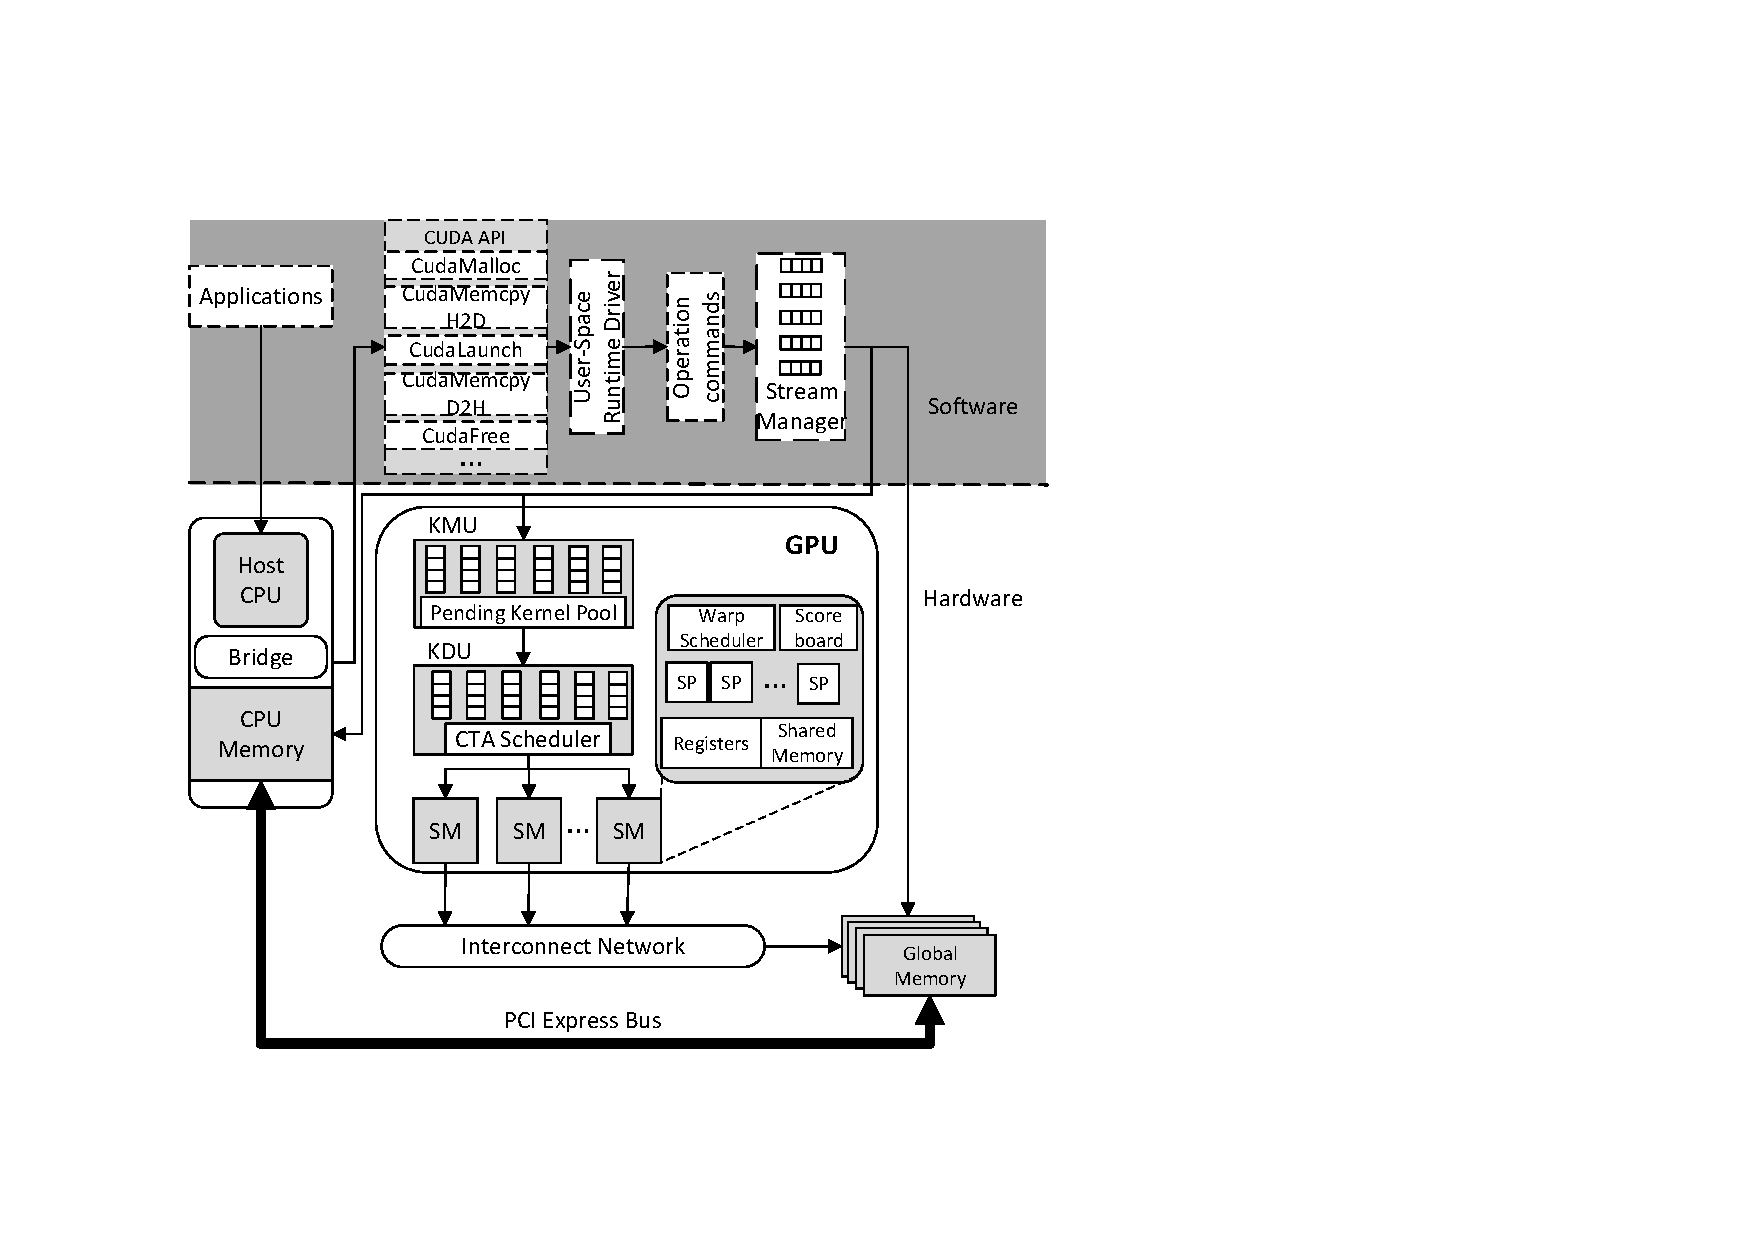
\includegraphics[width=\textwidth]{/Figs_PEP/Fig_Baseline_Architecture}
  \caption{GPU基准体系结构}
  \label{fig:Fig_Baseline_Architecture}
\end{figure}


\textbf{GPU体系结构}:图~\ref{fig:Fig_Baseline_Architecture}是GPU基准体系结构,我们本章所描述的GPU体系结构均基于此结构。
当一个GPU程序收到主机CPU执行时发送的操作指令,用户空间实时引擎将API调用指令转换为相关的GPU控制数据操作和内核函数的启动~\upcite{kato2011operating}。
GPU设备驱动发送这些操作指令到流控制管理器的队列里。
流控制管理器通过软件队列来管理多条不同的流(stream);每一条流里的指令将被串行执行。
一般来说,CPU会先声明并分配存储空间,然后调用cudaMalloc来分配GPU上的全局内存。
之后,一个cudaMemcpy(H2D)API的调用将数据从主机内存迁移到设备内存。
一旦所有的数据被传输完成,流控制管理器可以启动内核函数,即传输内核函数相关信息(例如维度配置和每个条目的PC地址)到内核函数管理器单元(Kernel Management Unit,KMU)。
当所有的信息准备完毕,内核函数会请求GPU核心资源。
如果内核函数没有获取足够的资源,则需要等待内核函数等待池有新的空间。
如果正在等待的内核函数的优先级高于正在执行的内核函数,则等待的内核函数有可能需要抢占GPU核心中正在占用资源的线程块。
否则,需要等待之前的内核函数执行完毕再接着执行。
一旦内核函数准备好开始执行,它将被传输到内核函数分发单元(Kernel Distributed Unit,KDU)。
线程块调度器将相应的线程块分发到不同的GPU核心。
每个GPU核心能够处理的线程块的最大数量取决于资源限制,包括可以执行的线程块数量、线程数量、寄存器数量和共享内存空间。
在每个GPU核心中的内核函数执行过程中,线程块将被分成warp,每个warp包含32或64个线程。
每个GPU核心包含一个或多个warp调度器,来选择执行哪一个warp。
在NVIDIA GTX 980 GPU系统结构中~\upcite{nvidia980s},每个warp调度器控制32个流处理单元(SP),每个流处理单元处理一个线程。
当一个warp因为访存或其他耗时较长的操作而停滞时,调度器会切换执行其他的warp。
切换warp没有任何开销,因为所有warp的上下文已经被放入寄存器和共享内存中。
因此,GPU通过掩藏停滞warp的延迟,显著提升了并行性能。

\subsection{先前的抢占方法}

当抢占发生时,每个GPU核心的操作是独立的。
这意味着有一部分GPU核心可能在执行抢占操作,而另一部分GPU核心在继续执行当前内核函数直到结束。
被抢占的GPU核心需要将该核内的上下文存储备份到全局内存。
一个GPU核心的上下文就是其执行的状态,包括SIMT栈、寄存器和共享内存。
SIMT栈存储的是线程执行信息,例如程序计数器和有效线程掩码(用于分支处理)。
相比于寄存器和共享内存的大小,SIMT栈的大小可以忽略不计,因此在本章我们暂不考虑SIMT栈。
一个线程块在其执行的时候占用GPU核心的资源;线程块保持活动状态直到其执行完毕。
但是,在其执行的时候,有可能有新的内核函数会被启动。
如果该新的内核函数需要满足严格的延迟要求,而等待上一个内核函数执行完毕再开始执行则无法满足该延迟要求。
因此我们需要去抢占一些正在运行的线程块来为新的内核函数的线程块提供资源。
但是,线程块的上下文相对来说非常大,将他们备份到全局内存将引入相当大的开销,抢占延迟也会非常大。
如表~\ref{table:time}所示,抢占延迟(平均上下文切换时间)有可能超过20$\mu$s。
这些延迟给需要满足延迟要求的新内核函数造成很大隐患。

为达到较低的抢占延迟的目标,Park等人提出了一种丢弃方法~\upcite{park2015chimera},在满足幂等性要求的前提下可以直接丢弃线程块,后续再重新执行。
在这个方法里,GPU核心直接丢弃掉线程块的上下文,并不备份相关上下文。
之后直接执行来自更高优先级内核函数的线程块。
在这个内核函数运行结束以后,GPU核心会重新开始执行被丢弃的线程块。
丢弃操作几乎没有抢占延迟开销。
但是,并不是所有的内核函数都能在任意时间执行丢弃操作。
丢弃操作要求内核函数是幂等的(Idempotent),这意味着该内核函数无论执行多少次,运行结果都是相同且独立的,即无原子操作,在丢弃操作发生之前无对全局内存的写操作。
大多数应用程序并不是幂等的(仅大约30\%的Rodinia应用程序满足幂等性条件)~\upcite{rodinia}。
幂等性可以变得相对宽松,但记录幂等性的开销非常大。
因此,实现丢弃操作的开销也可能非常大,与需要重复执行的指令成比例。

为了达到较低的抢占开销,GPU核心排空执行操作被提出。
该方法要求在新的内核函数的线程块开始执行之前,当前的线程块继续执行,直到结束~\upcite{tanasic2014enabling, park2015chimera}。
这种方法不要求上下文的存储备份,因此抢占开销能够最小化。
但是,这种情况的抢占延迟也可能非常高,这是因为内核函数的执行时间可能非常长,执行时间会非常长。
这很可能导致抢占内核函数无法满足其延迟要求。
表~\ref{table:time}包含了我们测量的不同的内核函数的单个线程块运行时间。
我们可以看到,有的线程块(如Kmeans)的执行时间达到接近1ms。
因此,GPU核心排空执行的方法最适合较短延迟的线程块。

Lin等人提出一种轻量化的上下文切换方法来减少需要备份到片外的上下文的大小~\upcite{lin2016enabling}。
这些技术主要包括本地上下文切换,将上下文存到未使用的寄存器或共享内存;
清除废弃的寄存器,即降低上下文大小;
还有寄存器压缩技术,我们在PEP中也采用了本地上下文切换技术。
但是,采用活跃度(liveness)信息要求为每一条指令的每一个寄存器提供一个活跃位(liveness bit),这将引入一个非常大的活跃度表存储在硬件里。
为降低这种较大的开销,抢占操作只能在特点的时间点执行,才能尽可能的使用较少的存储单元来存储活跃度信息。
而寄存器压缩技术也需要额外的硬件开销,因此我们也不在PEP中采用。

\subsection{GPU中的检查点备份技术}
检查点备份技术即是将一个运行的进程的状态备份的方法,目的是当出现错误时,能够从检查点恢复操作。
GPU检查点备份已经在软件上被实现~\upcite{takizawa2009checuda,nukada2011nvcr}。
虽然检查点备份能够恢复一个进程,但该技术的目的是容错,并不适合于抢占操作。
运行进程的设备有可能出现错误,所以有必要将运行状态存储到另一个设备。
这是一个非常高延迟的操作,但是相比于错误导致的工作进程丢失,这是非常必要的。
对于抢占操作,我们的目标是为抢占内核函数达到一个理想的反应时间,因为抢占内核函数需要满足一定的延迟要求。
因此,我们需要存储上下文到设备的全局内存。

我们的检查点备份技术并不是传统的面向容错处理的检查点备份技术。
实际上,这种上下文备份类似于检查点备份技术。
我们利用了检查点备份的技术在多任务抢占中降低需要存储的上下文的大小。
不同于传统的周期性的检查点备份,本章的检查点备份被采用来降低未来的上下文切换的延迟。
为引入检查点备份技术到抢占操作中,限制检查点次数尤为重要,因为我们另一个目标是降低抢占操作的开销。
PEP采用的检查点备份方法最多执行两次(一次初始检查点备份,一次增量备份)。
初始检查点备份有系统调用抢占内核函数的启动而触发,来自于硬件信号。
当前的检查点备份技术需要上下文的存储和错误恢复单元来保证可靠性,而我们的PEP检查点备份则是一种更加轻量化的方法,不要求任何错误恢复单元。




\begin{scriptsize}
\begin{table}[t]
\newcommand{\tabincell}[2]{\begin{tabular}{@{}#1@{}}#2\end{tabular}}
  \centering
  \begin{tabular}{|l|l|l|l|l|l|l|l|}  
    \hline
    \textbf{应用程序} & \textbf{内核函数} & \tabincell{c}{\textbf{平均}\\\textbf{启动}\\\textbf{时间}}  & \tabincell{c}{\textbf{平均}\\\textbf{线程块}\\\textbf{执行时间}} & \tabincell{c}{\textbf{平均}\\\textbf{切换}\\\textbf{时间}} & \tabincell{c}{\textbf{平均}\\\textbf{线程块}\\\textbf{大小}} & \tabincell{c}{\textbf{每个}\\\textbf{GPU核心}\\\textbf{线程块}\textbf{数量}}\\
    \hline
    \hline
    \tabincell{c}{CUTCP\\(CP)} & \tabincell{c}{cuda\_cutoff\\\_potential} & 5.8$\mu$s &516.2$\mu$s&10.1$\mu$s&16.5KB&8 \\
    \hline
    \tabincell{c}{LBM\\(LBM)} &  \tabincell{c}{performStream \\ Collide\_kernel} &21.8$\mu$s&31.7$\mu$s&20.9$\mu$s&18KB&14\\
    \hline
    \tabincell{c}{MRI-Q\\(MRI)}  &ComputeQ\_GPU&10.4$\mu$s&865.2$\mu$s&11.6$\mu$s&18KB&8 \\
    \hline
    \tabincell{c}{STENCIL\\(ST)}  & \tabincell{c}{block2D\_hybrid\\ \_coarsen} & 4.5$\mu$s&41.3$\mu$s&4.2$\mu$s&12.5KB&4 \\
    \hline
    \tabincell{c}{STREAM\\CLUSTER(SC)}  & \tabincell{c}{kernel\_ \\ compute\_cost} & 6.7$\mu$s & 605.6$\mu$s & 8.3$\mu$s & 24KB & 4\\
    \hline
    \tabincell{c}{GEMM\\(GM)}  & matrixMulCUDA & 23.4$\mu$s &193.6$\mu$s& 17.9$\mu$s&28KB&8\\
    \hline
    \tabincell{c}{BLACK\\SCHOLES(BS)} & BlackScholarGPU &3.4$\mu$s & 387.5$\mu$s & 16.7$\mu$s&12.5KB&16 \\
    \hline
    \tabincell{c}{KMEANS\\(KS)} & invert\_mapping & 29.7$\mu$s & 984.7$\mu$s & 9$\mu$s&10KB&8\\
    \hline
    \tabincell{c}{PATHFINDER\\(PF)}  & dynproc\_kernel&11.3$\mu$s &24.2$\mu$s&11.6$\mu$s&18KB&8\\
    \hline
    \tabincell{c}{SRAD\_V1\\(SRAD1)} & extract&5.2$\mu$s &1.8$\mu$s&4$\mu$s&12KB&4\\
   	\hline
    \tabincell{c}{SRAD\_V2\\(SRAD2)}  & srad\_cuda& 15$\mu$s & 11.5$\mu$s&16.4$\mu$s&25KB&8\\
    \hline
    \tabincell{c}{SRAD\_V1\\(SRAD3)} & srad & 5.2$\mu$s &7.9$\mu$s &7.8$\mu$s&24KB&4\\
    \hline
    \tabincell{c}{HOTSPOT\\(HS)} & calculate\_temp &33.3$\mu$s&4.5$\mu$s&7.7$\mu$s&38KB&3\\
    \hline
    \tabincell{c}{LUD\\(LUD)} & lud\_internal & 4.4$\mu$s &5.3$\mu$s&10.5$\mu$s&16KB&8\\
    \hline
    \tabincell{c}{BACKPROP\\(BP)} & \tabincell{c}{bpnn\_ \\ layerforward} & 16.7$\mu$s &4.7$\mu$s &2$\mu$s&12KB&1\\
    \hline
    \tabincell{c}{BACKPROP\\(BP2)} & \tabincell{c}{bpnn\_adjust \\ \_weights} & 16.7$\mu$s & 1.5$\mu$s &1.2$\mu$s&22KB&1\\
    \hline
    
  \end{tabular}
  \caption{各应用程序启动时间、线程块切换时间与执行时间}
  \label{table:time}
\end{table}
\end{scriptsize}

\section{研究动机}
\label{sec:pepmotivation}

Chimera~\upcite{park2015chimera}采用了一个选择算法在抢占请求到来时为不同的线程块选择不同的抢占方法;这个选择是基于对前面介绍的三种方法的选择和平衡。
Chimera估计了每一种技术的抢占延迟和开销来选择最有效的抢占方法。
因此,GPU核心中不同的线程块会被不同的抢占方法被抢占。

但是我们发现排空执行方法和上下文切换方法会竞争全局内存的带宽。
举例来看,在图~\ref{fig:motivation}中,访存密集型的应用程序LBM会遇到这样的一种冲突:
LBM在每个GPU核心中可以执行9个线程块;我们展示了所有10种切换和排空执行的可能性组合。
如果所有的线程块被一个接一个地切换,则不会出现切换和排空执行的竞争。
而另一种情况是当一个GPU核心在上下文切换时,其他GPU核心都在排空执行时,排空执行的时间和上下文切换时间都将远长于8个线程块在做上下文切换操作,1个线程块在排空执行的情况。
因此,我们发现带宽竞争会导致Chimera时间估计不准确的问题。
在这种情况下,当1个线程块在排空执行时,其他线程块一个接一个被切换时带宽竞争非常小。
另一方面,这个排空执行的线程块不会与其他线程块竞争执行单元。
因此,单位时间执行的平均指令数(IPC)受到排空执行的线程块的数量影响。


\begin{figure}[htbp] % use float package if you want it here
  \centering
  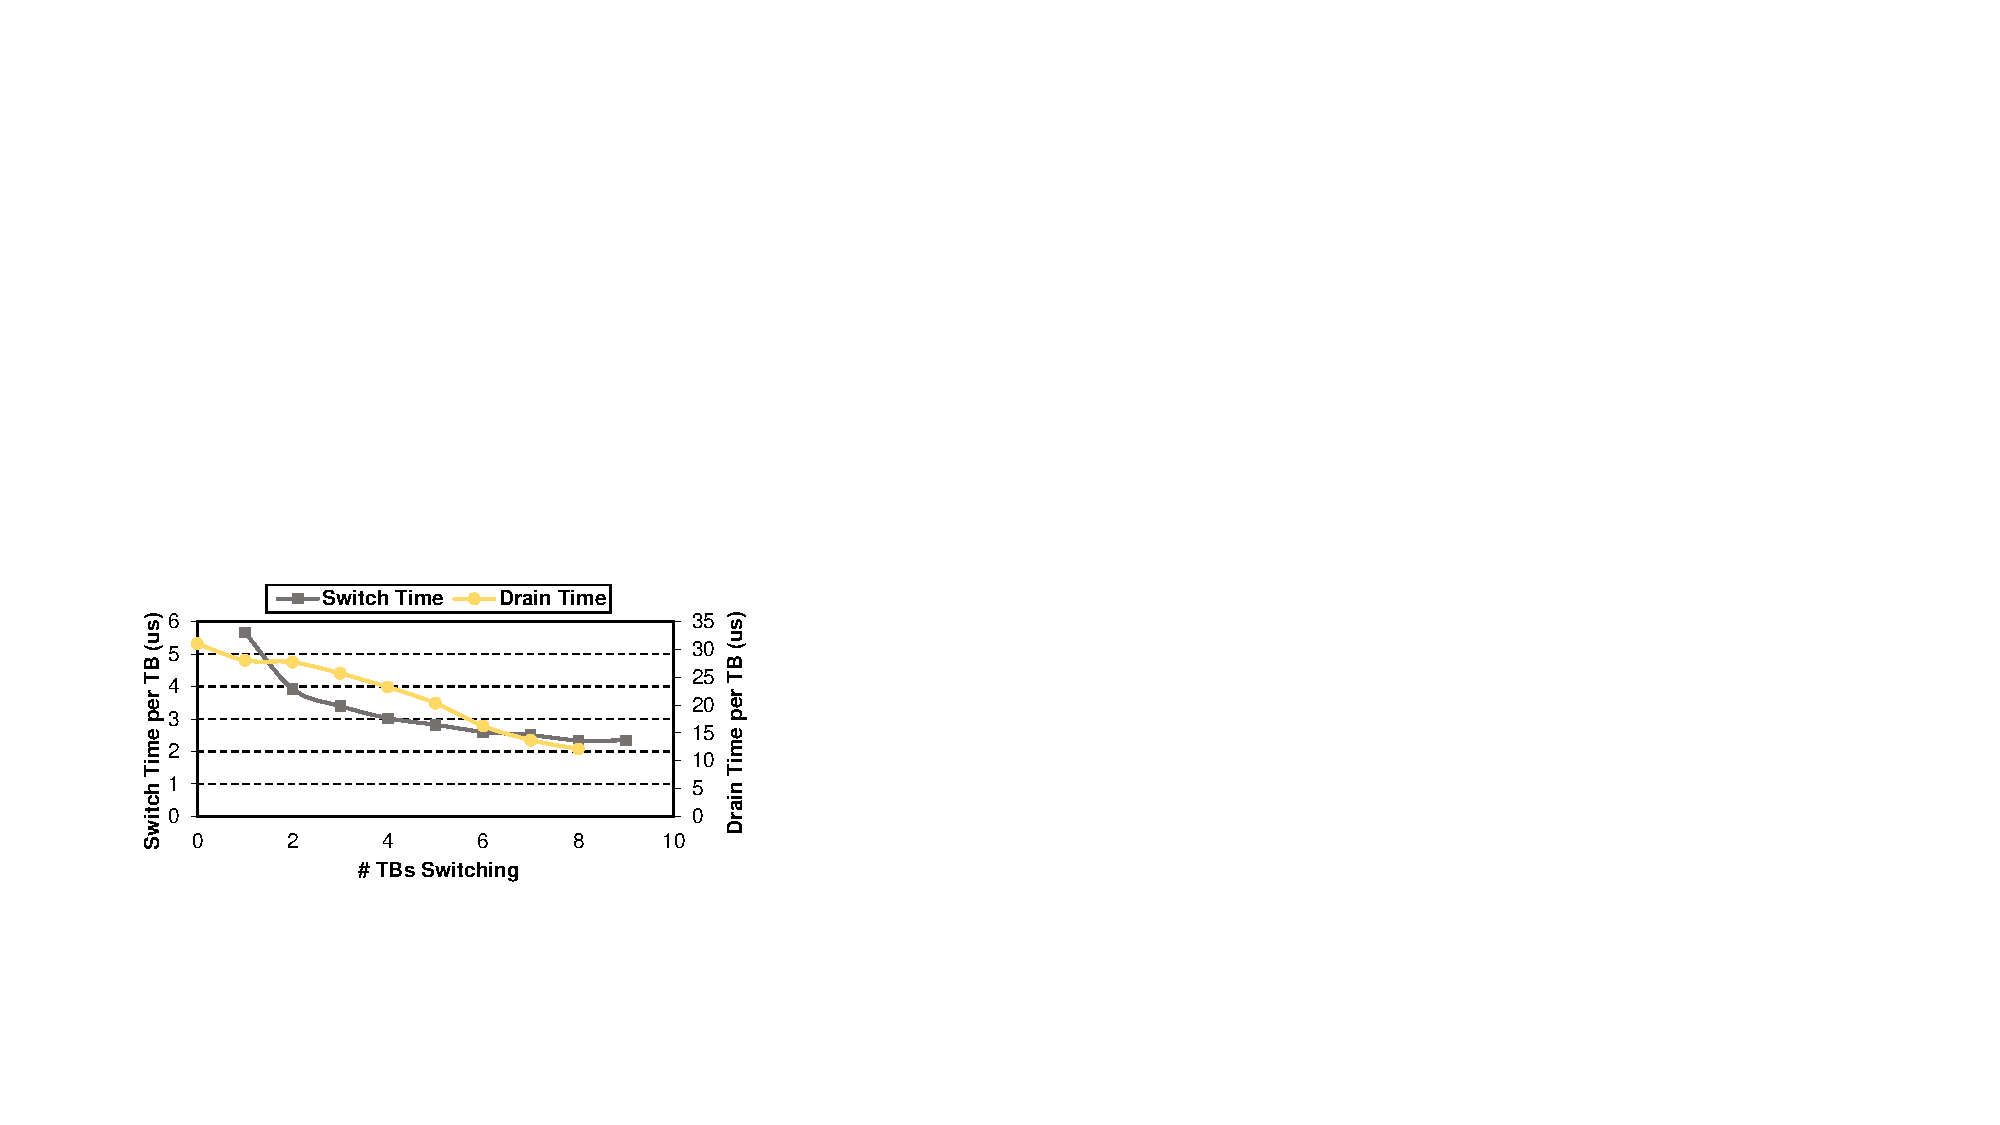
\includegraphics[width=.7\textwidth]{/Figs_PEP/motivation}
  \caption{LBM的上下文切换时间和排空执行时间对比(每个GPU核心有9个线程块在同时执行)}
  \label{fig:motivation}
\end{figure}


我们也观察到在每个GPU核心中所有的线程块通常选择同一种抢占方法。
表~\ref{table:time}展示了线程块执行时间的范围远大于上下文切换的时间范围。
因此,对于长内核函数,排空执行时间和上下文切换时间相差巨大。
而对于短的抢占内核函数来说,最佳方法是排空执行GPU核心内所有的线程块,这可以满足延迟要求的同时接近零抢占开销。
相反,对于长的内核函数,如果不满足幂等性要求,则必须做上下文切换。

当前GPU~\upcite{pascal}的总上下文大小是每个GPU核心有352KB(寄存器包含256KB,而共享内存包含96KB)。
为了传输所有上下文到全局内存,假设带宽被完全利用需要大约15$\mu$s。
之前所有的技术都是被动的,他们至少需要这么长时间来完成上下文切换。
为了进一步降低上下文切换的抢占延迟,我们不仅需要减少上下文的大小,还需要一种主动的抢占方法。

检查点备份技术即是一种主动机制广泛应用于容错处理中。
该方法周期性地存储当前进程的执行状态到下一级存储中。
类似地,我们可以针对抢占操作,将正在运行的线程块的上下文存储到全局内存中。
我们介绍一种新的检查点方法,称之为PEP。
PEP在抢占发生之前将当前检查点的上下文备份,当真正的抢占操作开始后,我们只需要被动地存储这段时间更新的上下文,这显著减少了抢占等待时间。

\section{相关工作}
\label{sec:peprelated}

检查点备份技术主要用于容错处理上~\upcite{teodorescu2006swich,li2017fine}。
传统的检查点软件,如\emph{BLCR}~\upcite{hargrove2006berkeley},支持通过自定义的Linux内核执行检查点备份CPU的状态。
这并不能在CPU片外的GPU工作,因为GPU的内存是通过设备驱动程序操作的。
因此,\emph{BLCR}不能恢复其状态。
\emph{CheCUDA}~\upcite{takizawa2009checuda}是第一个尝试去解决NVIDIA GPU上的这个问题。
它作为一个\emph{BLCR}的附加组件实现,可以与BLCR一起工作,但要求重新编译应用程序。
\emph{NVCR}~\upcite{nukada2011nvcr}进一步提升该方法,支持使用实时API的更大集合类的应用程序。
它替换了\emph{libcuda.so},因此,不需要重新编译应用程序。
此外,虚拟化是另一个采用了检查点备份技术的应用。
vCUDA~\upcite{shi2012vcuda}则是一个GPU虚拟化方面的重要工作。



所有之前的抢占工作都是被动的,意味着这些机制都是在抢占内核函数启动并要求资源后才会被触发。
因此,任何算法都需要等待GPU核心的上下文切换完成或者排空执行完成。
我们通过利用内核函数启动过程的特点,PEP设计了一种主动触发技术。
利用检查点备份方法,PEP可以实现一个相对于其他方法更短的呃抢占延迟,同时开销可控。

\section{主动抢占策略的设计}
\label{sec:pepdesign}

在本节中,我们首先给出了主动抢占设计的全局概要图。
然后我们将证明预测内核函数启动时间和估计抢占时间的可行性。
最后,我们提出了基于检查点方法的设计和在线选择算法。

\subsection{全局设计}
我们的方法是来源于一个观察:只要延迟和开销是可以接受的,上下文切换可以在线程块执行的任何阶段发生。
为了降低延迟和开销,我们将减少上下文的大小。
为了减少抢占延迟,我们可以提前做上下文切换。
在合适的时机我们采用了排空执行的方法,因为这个方法几乎没有开销。

为了减少上下文的大小,我们采用了脏位来指明一个寄存器是否被写过。
因此,我们不会存储未使用或者已经被释放的上下文。
我们还会采用Lin等人提出的本地上下文备份的方法~\upcite{lin2016enabling},该方法支持让上下文存入空闲的本地内存。
在这个方法中,不需要通过互连网络将数据传输到全局内存,因此不占用存储带宽。

采用检查点备份技术来实现主动上下文切换。我们的算法支持在抢占之前的某个检查点存储数据到全局内存。
接着继续执行当前内核函数,直到抢占请求到来。
此时,我们只需要将这段时间相对于上一个检查点的上下文增量更新存储到全局内存中。
如果一个线程块在初始检查点和抢占发生直接执行完成,则释放初始检查点存储的上下文。
这个方法可以取得远小于一次完整上下文存储的开销。

为了在抢占中实现检查点备份,我们必须限制检查点存储发生的次数。
如果我们备份太多次检查点状态,开销很可能无法接受。
另一方面,如果一个线程块在多个检查点之后,抢占之前执行完毕,则之前的检查点备份均浪费掉了,同时还耗费了不少开销。
因此,我们有必要预测线程块是否能在抢占点发生的时候依然在执行。
此时,我们只需要为在抢占发生时依然在执行的线程块执行检查点备份。
我们知道内核函数在GPU的执行是在CUDA API调用cudaLaunch之后发生的。
在这个API调用之后,一个内核函数启动的命令将被发送到流控制管理器中。
如果这个命令进入流队列的队列头,内核函数的相关信息将被发送到内核函数管理单元,开始请求GPU核心资源。
因此,我们发现内核函数启动的时间是可以被预测的。

我们的检查点备份非常适合长内核函数。
对于短的内核函数,我们还是会采用排空执行的方法代替上下文切换。
为了采用这两种抢占技术,我们需要估计排空执行和上下文切换的时机以在线选择合适的抢占方法。

\subsection{预测和估计}
内核函数启动时间的预测和排空执行时间和上下文切换时间的估计是PEP的关键部分。
通过对一系列应用程序的研究分析,我们发现有三个时间对我们预测策略的正确性特别关键,分别是内核函数启动时间、上下文切换时间和线程块执行时间。
内核函数启动时间可以用来预测什么时候抢占请求会真正启动。
上下文切换时间和线程块执行时间可以用来确定采用基于检查点的上下文切换技术还是排空执行技术。
表~\ref{table:time}展示了我们测量的三种延迟。

1)\textbf{预测}:从对表~\ref{table:time}的研究有两点重要的观察。
第一,是我们发现内核函数启动的时间和上下文切换的时间(接近检查点备份的延迟)是在同一个数量级。
这意味着如果我们在开始在预测的时间进行一次检查点备份时,很可能在抢占请求发生时,我们刚好完成有效上下文的存储备份。
第二,无论是上下文切换时间还是内核函数启动的时间,在大多数情况都远小于线程块的执行时间。
对于长内核函数的线程块,不太精确的预测不会影响我们是做检查点备份还是排空执行。
因此,一次错误的预测不会对最终的延迟性能和开销造成巨大影响。
我们将在本节详细讨论这些延迟信息。

前面已经提到,我们必须预测何时抢占请求会出现以避免检查点备份作废。
一个CUDA应用程序一般包括5个步骤,我们将其概括为5个重要的CUDA API调用,包括cudaMalloc、cudaMemcpy(H2D)、cudaLaunch、cudaMemcpy(D2H)和cudaFree。
cudaLaunch会触发内核函数启动。
该操作会将内核函数的相关信息传输到GPU,包括线程块的组织信息(网格和块的维度)、指针以及共享内存的分配等信息。
我们测试了大量的应用程序,观察到内核函数启动的时间是在几十微秒的数量级。
表~\ref{table:time}展示了一系列我们测试的应用程序,可以发现内核函数启动时间从3.3$\mu$s到33.3$\mu$s不等。
这个时间是从cudaLaunch被调用到内核函数信息被传输到内核函数管理单元,假设没有在流控制处理器中排队。
这种较高的内核函数启动时间包括软件API调用和参数数据拷贝到GPU的内核函数等待池(Pending Kernel Pool)的过程~\upcite{puthoor2018oversubscribed}。
因此,这些开销会有很大差异。

此外,每个线程块的平均上下文切换时间从1$\mu$s到20$\mu$s不等,该时间取决于每个线程块的上下文的大小。
从表~\ref{table:time}可知,上下文切换的时间和内核函数启动的时间在同一个数量级。
上下文切换的时间大致与内核函数启动的时间接近。
这意味着初始检查点备份完成,抢占请求可能已经启动。
在这种情况,可以立即释放资源,为新的内核函数腾出空间。
我们的设计不要求对内核函数启动时间的精确预测。
这是因为如果一个检查点备份完成之后,真正的抢占请求还未到来。
GPU核心可以继续执行线程块直到抢占开始,在抢占时仅需存储更新的上下文。

如表~\ref{table:time}所示,我们也发现平均线程块的执行时间再1.5$\mu$s到超过900$\mu$s不等。
这种变化不定的线程块执行时间完全取决于内核函数的大小。
短内核函数的线程块将被排空执行。
这种方法几乎没有开销,同时满足抢占内核函数的延迟要求,因为排空执行的时间非常短。
只有长内核函数的线程块需要进行上下文切换的操作。
因为那些大的线程块的执行时间可以达到几百微秒,因此在内核函数启动的API被调用时粗略地预测一个线程块是否会被抢占并不难。
为了实现预测的目的,我们设置内核函数启动的时间为20$\mu$s。
当一个cudaLaunch被调用,我们比较预测的内核函数启动时间和每个线程块的剩余执行时间。
如果预测的内核函数启动时间小于线程块的执行时间,则我们立刻采用检查点备份技术执行上下文切换。
否则,我们将采用排空执行该线程块。
注意到与线程块执行时间相比,内核函数启动的时间相对变化较小。
因此,即使一个内核函数的真正启动时间不是20$\mu$s,也不太可能导致我们选择其他的抢占方法。

现实情况中,内核函数启动的时间可能会因为在流控制处理器中的队列等待而延迟。
例如,之前的一个长的内存拷贝操作仍然没有结束,堵住了流控制处理器的队列。
但是这个延迟在我们的算法中并不是个问题。
在平均线程块执行时间远大于内核函数启动时间的情况,例如对于CUTCP,这个延迟不太可能比线程块完成执行的时间还快,所以我们的检查点策略不会被浪费。
而在平均线程块执行时间小于内核函数启动时间的情况,我们会选择排空执行,所以这个延迟也确定不会影响检查点备份的开销。

我们的预测方法将确定检查点备份的总次数不会超过两次。
初始检查点备份被cudaLaunch调用来触发,而增量检查点备份被抢占请求触发。
因此,检查点备份的开销是可以被控制的。

2)\textbf{时间估计}:我们可以估计上下文切换的时间和排空执行的时间来选择不同的抢占策略,即基于检查点备份的上下文切换和排空执行。
我们还需要时间估计来预测抢占是否在当前线程块执行的时候发生。
Chimera~\upcite{park2015chimera}采用时间估计的方法来比较不同的抢占方法的吞吐量开销。
Chimera估计每个线程块的排空执行时间为线程块剩余的指令数乘以该线程块之前的CPI。
上下文切换时间为每个线程块的上下文大小除以全局内存被每个GPU核心分享的带宽。
但是这种基于线程块的方法在某些情况下并不准确。
而当排空执行和上下文切换同时进行的时候,这个时间变得无法估计。
如图~\ref{fig:CDrain_Est}所示,当一般的线程块在排空执行,而其他的线程块在做上下文切换时,估计的时间与实际的时间相差巨大。
这是因为较少的排空执行的线程块意味着在流处理器(SP)较小的冲突,上下文切换的线程块在全局内存的带宽上出现更多的冲突。


\begin{figure}[htbp] % use float package if you want it here
  \centering
  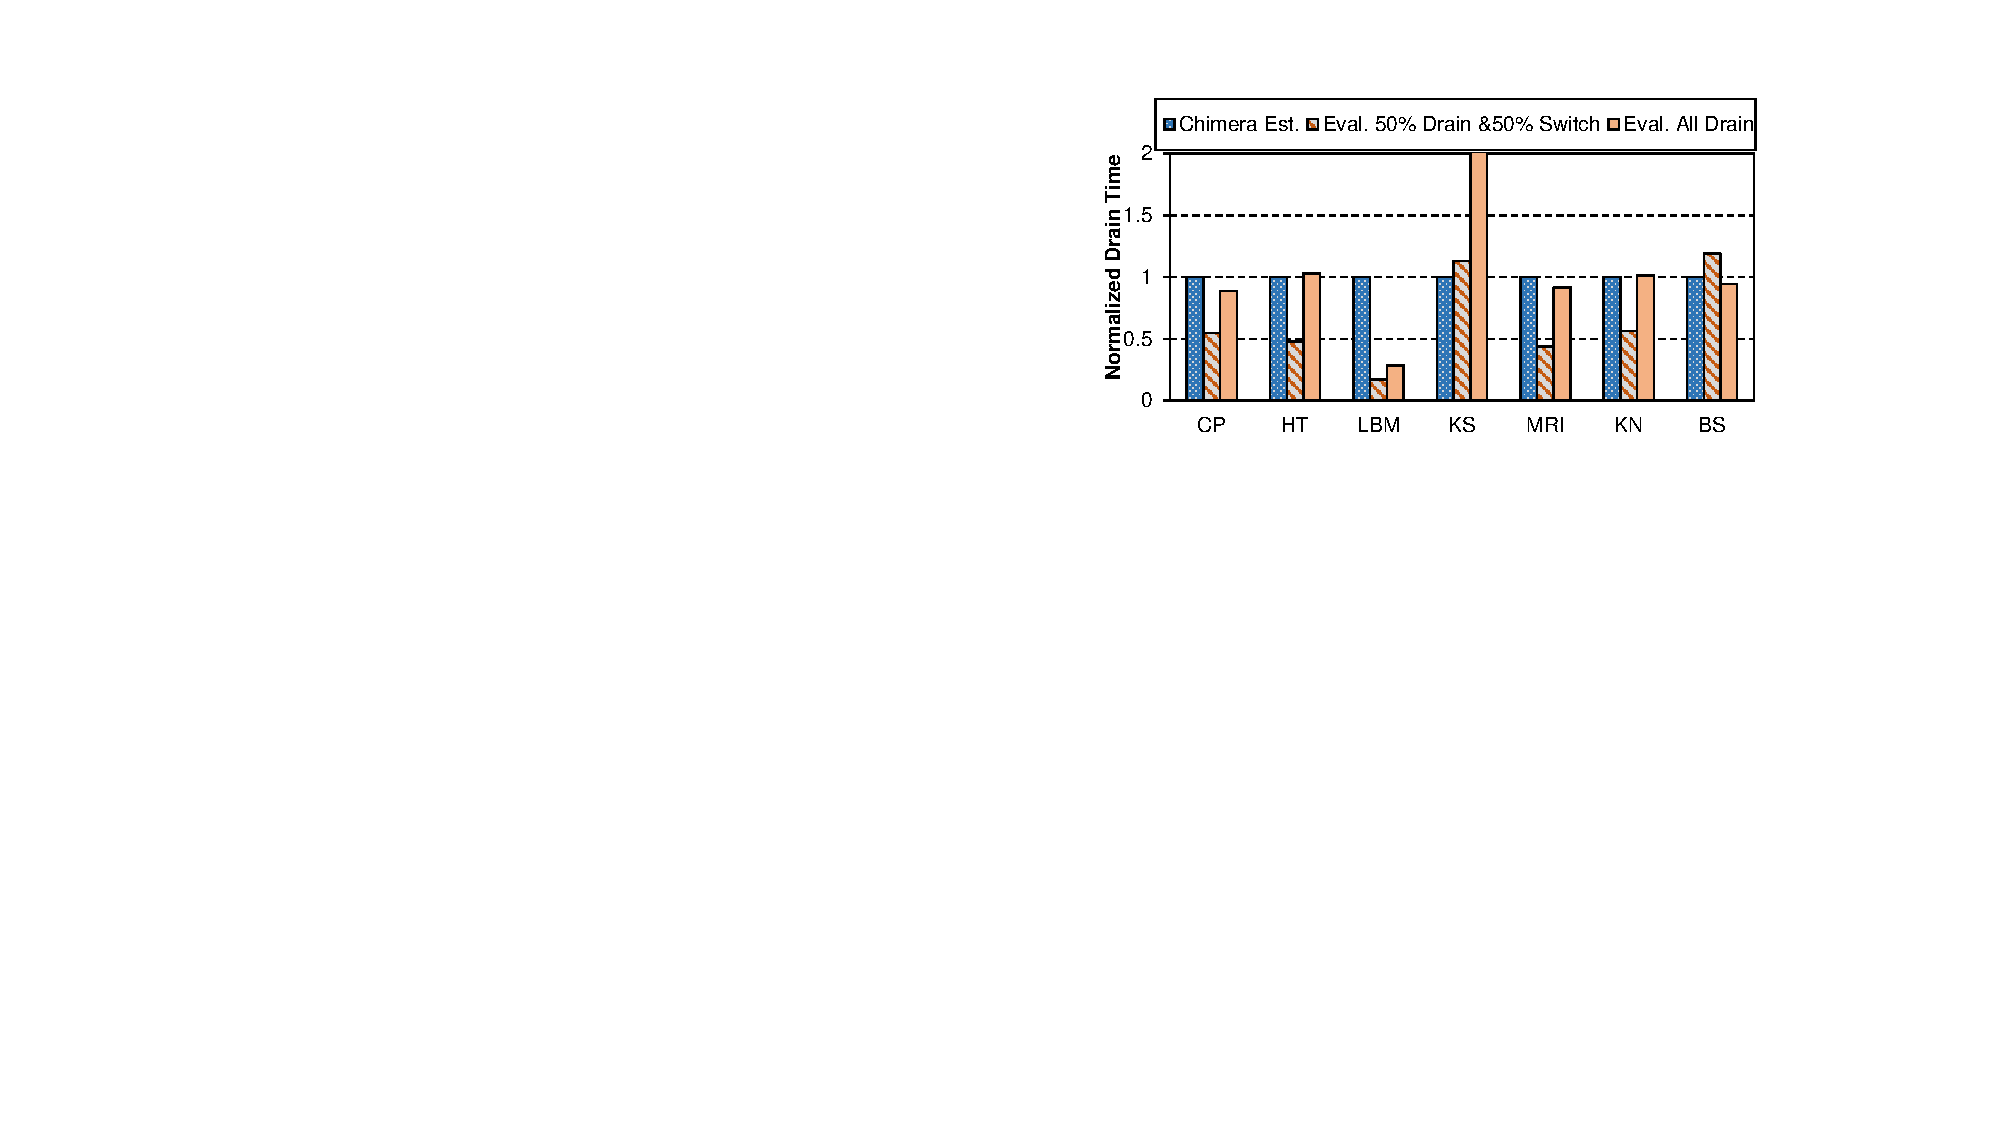
\includegraphics[width=.8\textwidth]{/Figs_PEP/CDrain_Est}
  \caption{Chimera的估计排空执行时间}
  \label{fig:CDrain_Est}
\end{figure}


虽然Chimera的估计对于全部线程块都做排空执行时更加精确,在某些特定情况仍然有非常不精确的地方。
比如说,有的应用程序,如LBM和KS有多个阶段:它们的CPI在不同的时段不一样。
在图~\ref{fig:CDrain_Est}中,KS在开始的时候CPI非常低,但其CPI随着程序的执行而不断上升。
因此,估计的时间和真实测量的时间相差很大。
另外,Chimera估计上下文切换时间来选择抢占策略时,只考虑单个线程块。
例如三个线程块在做上下文切换,则需要传输备份的总上下文大小是原上下文大小的三倍。
因此真正的上下文切换时间要比Chimera估计的每个线程块上下文时间长3倍。

从表~\ref{table:time}中可知,线程块的执行时间和线程块的上下文切换时间相差很大。
对于大多数的应用程序,我们会选择排空执行所有的线程块或者上下文切换所有的线程块。
因此,排空执行的时间和上下文切换的时间是可估计的。
我们不需要担心上下文切换和排空执行的互相干扰。
为了避免CPI随时间变化的影响,我们在线收集线程块的执行时间。
由于不同的线程块执行的指令在大多数情况都是相同的,所以线程块的执行时间是相对稳定的。
因此,可以采用之前收集的平均线程块执行时间减去已经执行的时间以获取线程块的剩余执行时间。
所以,如果在需要估计执行时间的时候还未收集到线程块的执行时间,将采用Chimera的时间估计方法。
为了估计上下文切换的时间,本章采用了最坏情况来估计,即估计的时间为当前GPU核心所有线程块被上下文切换出去的时间。
由于上下文切换的时间范围小于线程块的执行时间,我们使用最坏情况来估计比较有保证。


\subsection{上下文缩减}
传统的上下文切换将所有分配的上下文存储都全局内存中。
但是,在某一个特定的时间点活跃的上下文总是小于分配的大小,这使得需要存储备份的上下文大小相对较少。
本章采用脏位实时追踪活跃的上下文。
但是,线程块主要有两种上下文,寄存器和共享内存。
他们的声明周期是不同的。共享内存时每个线程块私有的。
由于这是被程序员来管理的,我们将共享内存的生命周期当成线程块的生命周期。
另一方面,寄存器是分配给每一个线程的,并且是在每一个warp中同时执行。
因此,一个寄存器的生命周期与warp有关。当一个warp结束后,所有这个warp相关的寄存器将被完全释放。
为了追踪寄存器的利用率,在写回的过程中,一旦一个寄存器被写入数据则需要置脏位为1。
当warp运行完成或者检查点备份后将重置相应脏位,可以用类似的方法追踪共享内存写。

图~\ref{fig:dirtyrate}展示了多个应用程序的脏寄存器的大小相比于被分配的大小。
我们收集了不同执行阶段脏寄存器的百分比。
我们的初始收集点是线程块执行的25\%阶段。
Dirty1和Dirty2是脏寄存器在50\%和75\%线程块执行时间相比于初始收集点的百分比。
对于一些包含了非常多指令的内核函数,MRI到PF,Dirty1和Dirty2相比于初始状态,平均下降了38.2\%和48\%。一般来说,Dirty2相比于Dirty1有较少的脏寄存器,因为在75\%的时间点部分warp执行结束,并释放了一些寄存器。我们发现这样的脏位分析是足够的,我们不需要采用编译时的活性分析和寄存器值的压缩。

\begin{figure}[htbp] % use float package if you want it here
  \centering
  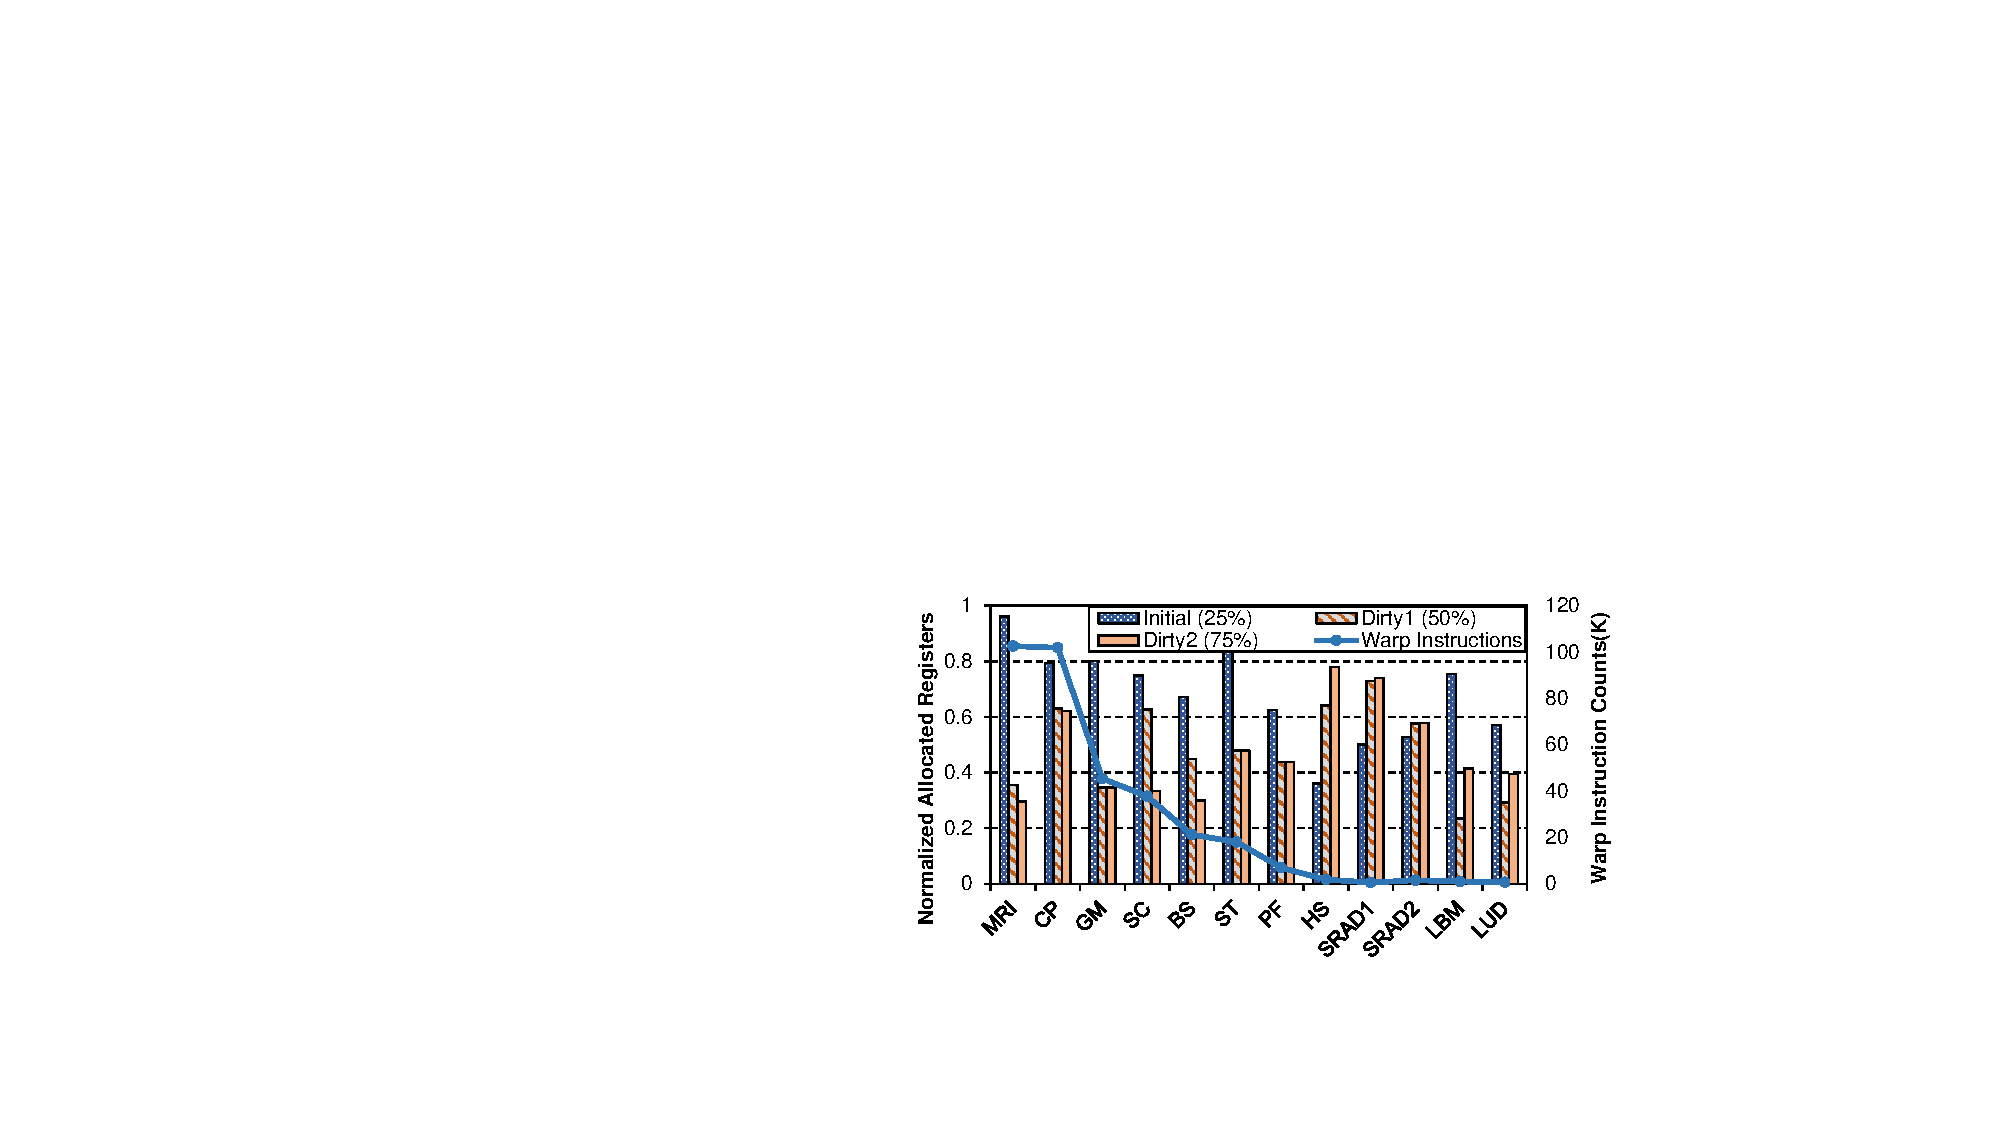
\includegraphics[width=.8\textwidth]{/Figs_PEP/dirtyrate}
  \caption{相对于分配的寄存器数量:Initial:线程块执行时间的25\%、Dirty1: 线程块执行时间的50\%、Dirty2:线程块执行时间的75\%}
  \label{fig:dirtyrate}
\end{figure}


我们还在增量检查点备份中采用了本地上下文存储~\upcite{lin2016enabling}。
因为新的内核函数可以采用旧内核函数没有使用的空间,本地上下文切换的方法得以采用。
这将进一步降低实际的抢占延迟。

\subsection{主动抢占方法设计}

1)\textbf{检查点备份}:检查点备份只在大的被抢占的内核函数中被使用,因为他们排空执行的时间过长。
当一个内核函数在多个GPU核心上运行时,如果一个cudaLaunch被调用,我们知道新的内核函数将要在几十个微秒内被传输到GPU。
在这个时候,GPU驱动将发送一个信号来激活微程序化陷阱程序~\upcite{menychtas2014disengaged}。
这是通过命令队列和存储映射寄存器~\upcite{gpuvm}。
当前的GPU通过一些可以被开发者直接访问的寄存器来激活抢占操作,但并不是被终端用户来激活。
当检测到一个抢占内核函数启动的请求,则一个初始检查点备份命令被写入命令队列,之后会修改存储映射的寄存器来开始每个GPU核心的检查点备份~\upcite{suzuki2016gpuvm}。
我们测量了NVIDIA GTX 1060 GPU的信号传输时间。
这个延迟大约在1.3$\mu$s,对于不同的应用程序这个值也相对稳定。
这个信号将触发一次检查点备份。
我们将暂停取新指令,然后开始完成流水线指令。
否则,在检查点备份上下文的时候,上下文也在持续变化。
如果当前的内核函数是计算密集型的,完成流水线指令的过程需要几十个时钟周期。
如果当前的内核函数是访存密集型的,我们必须等待访存请求返回来完成流水线上的指令。
因此每个GPU核心中执行完所有流水线上的指令需要几百个时钟周期。
初始检查点需要备份的上下文是相对于初始状态的脏寄存器和共享内存。

当检查点备份完成后,所有的脏位将被重置。
之后,GPU检查是否有新的内核函数被传输到内核函数管理单元。
如果内核函数在内核函数等待池,则一旦获得GPU核心资源则可以开始执行。
则当前内核函数可以被立刻抢占,因为当前的执行状态已经被存储。
否则,当前内核函数需要继续执行直到真正的抢占请求到来。
当真正的抢占请求到来时,我们只需要存储变化的上下文。
因为这一次检查点备份的上下文是相对于上一次检查点备份变化的部分,因此需要备份的上下文非常小,消耗的时间也短很多。
因为只有变化的上下文需要被存储,没有重复的数据需要被存储。
综上所述,当新的高优先级的内核函数的cudaLaunch被调用时,初始检查点备份将开始。
因此,新内核函数很快被调用。
所以,增量检查点备份的上下文肯定会非常小。
除此之外,由于本地上下文存储的利用,需要被存储的上下文的大小可以进一步减少。

被抢占的内核函数的恢复和传统的检查点恢复类似。
如果我们有两次检查点状态需要恢复,则必须先恢复后一次的状态再恢复前一次的状态。
但是,在这个时候GPU核心不允许执行任何任务。
所以,所有的带宽将被用来做上下文恢复。

\begin{figure}[htbp] % use float package if you want it here
  \centering
  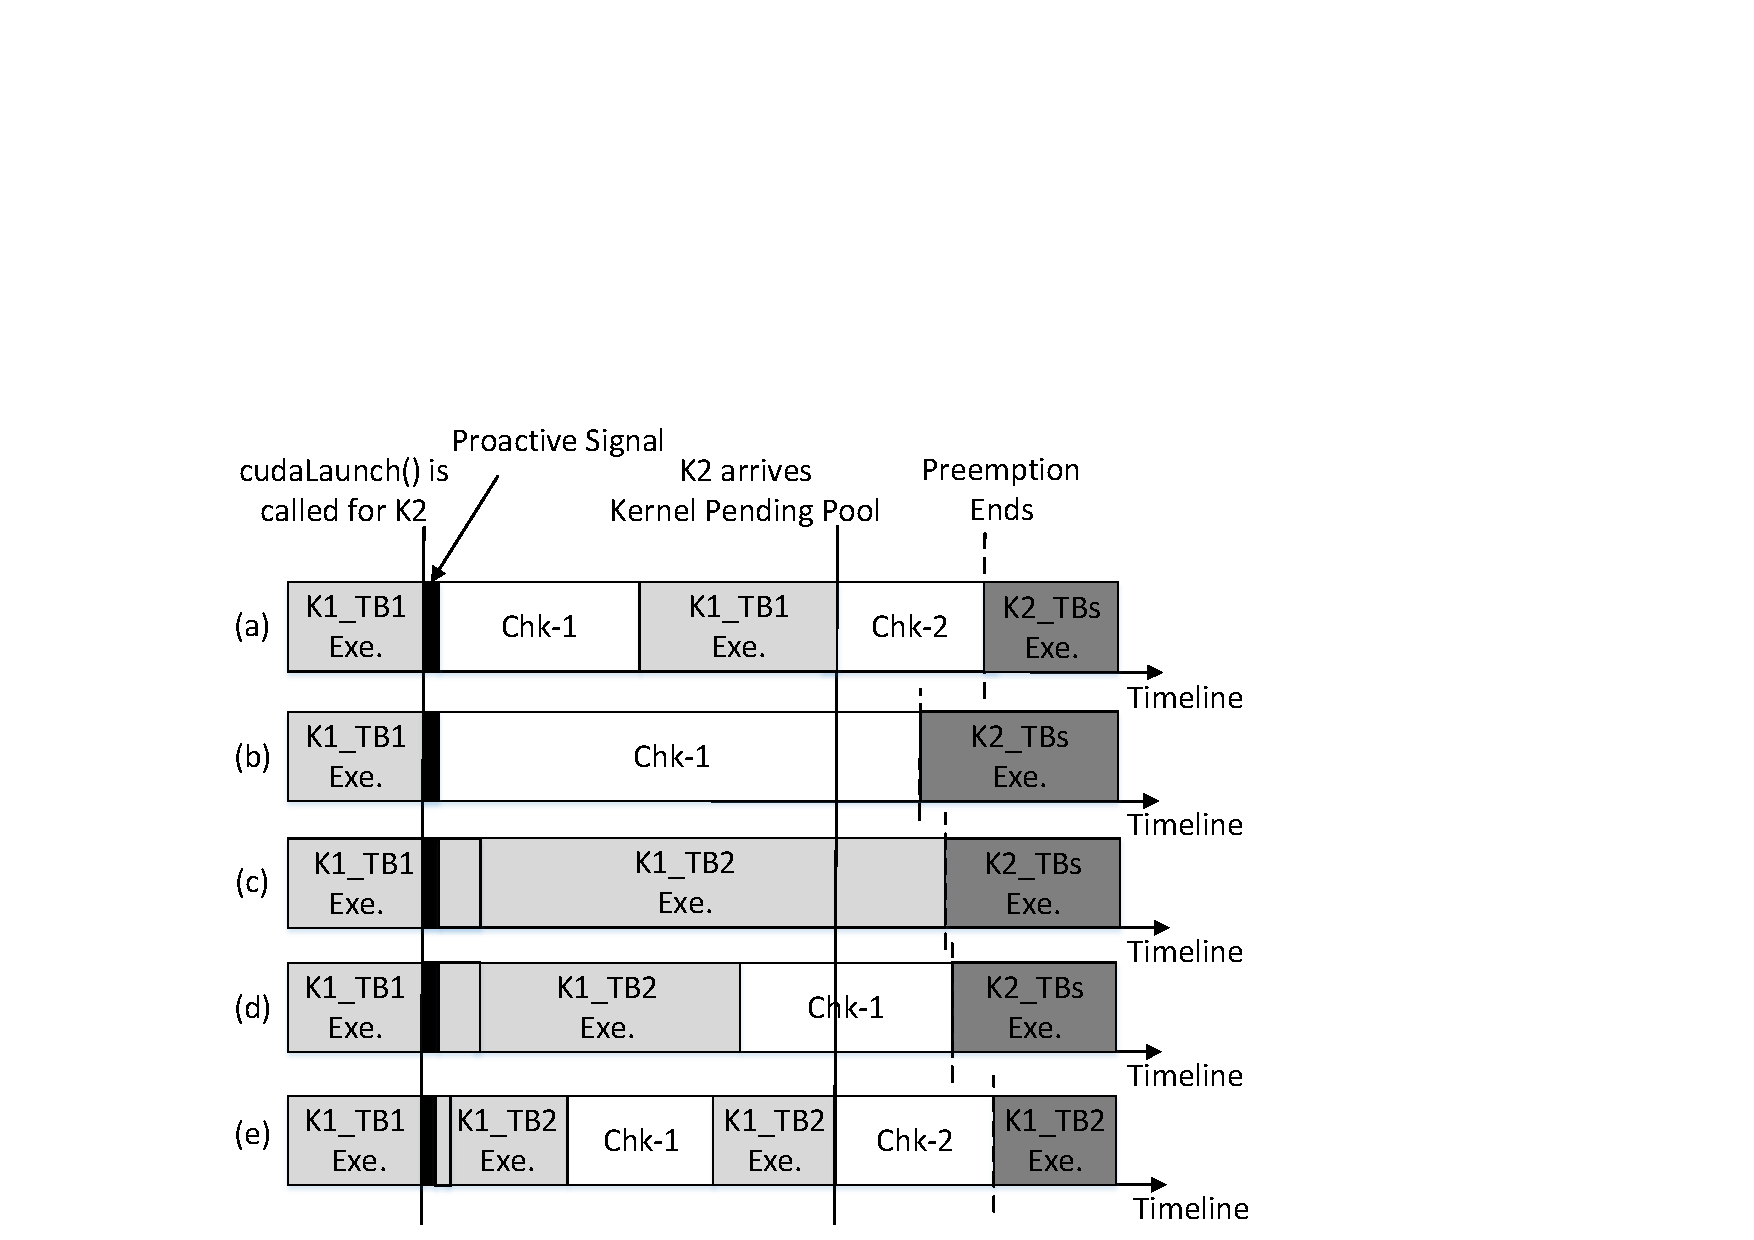
\includegraphics[width=\textwidth]{/Figs_PEP/allconditions}
  \caption{PEP可能性分析:K1:被抢占的内核函数、K2:抢占内核函数、Chk-1:基本检查点备份、Chk-2:增量检查点备份}
  \label{fig:allconditions}
\end{figure}


2)\textbf{在线选择器}:从表~\ref{table:time}中我们可以知道,执行时间、上下文的大小还有内核函数启动时间对于不同的内核函数都不一样。
因此,当cudaLaunch触发了我们的主动抢占机制,有许多种可能性。
图~\ref{fig:allconditions}展示了这些可能性:


\renewcommand*\theenumi{(\alph{enumi})}
\begin{enumerate}
\setlength\itemsep{1pt}
\item 两次检查点备份:这是最常出现的情况。
内核函数启动的时间比初始检查点备份的时间长。
当真正的抢占请求到来的时候,我们再将更新的上下文做一次增量备份。

\item 单次检查点备份:这实际上和传统的上下文切换是一样的,但是这个检查点备份比传统的上下文切换更早发生。

\item 排空执行:这种情况被抢占的内核函数比较小。
线程块的执行时间比抢占内核函数的启动时间要小,很可能会在延迟限制前完成。
在这种情况,我们排空执行所有的线程块来达到极小的开销。

\item 排空执行然后单次检查点备份:被抢占的内核函数和(b)的情况一样。
如果一个线程块接近执行完毕,则抢占不会发生在当前线程块的执行过程中。
因此,我们会先排空执行线程块,然后当新的线程块被发送到这个GPU核心。
新的线程块会开始执行一定数量的指令后开始检查点备份。本章我们设置这个指令的数量为1000.

\item 排空执行然后两次检查点备份。
被抢占的内核函数和(a)的情况一样。
当cudaLaunch被调用时,线程块接近执行完毕,和d的情况类似。
\end{enumerate}


\begin{figure}[htbp] % use float package if you want it here
  \centering
  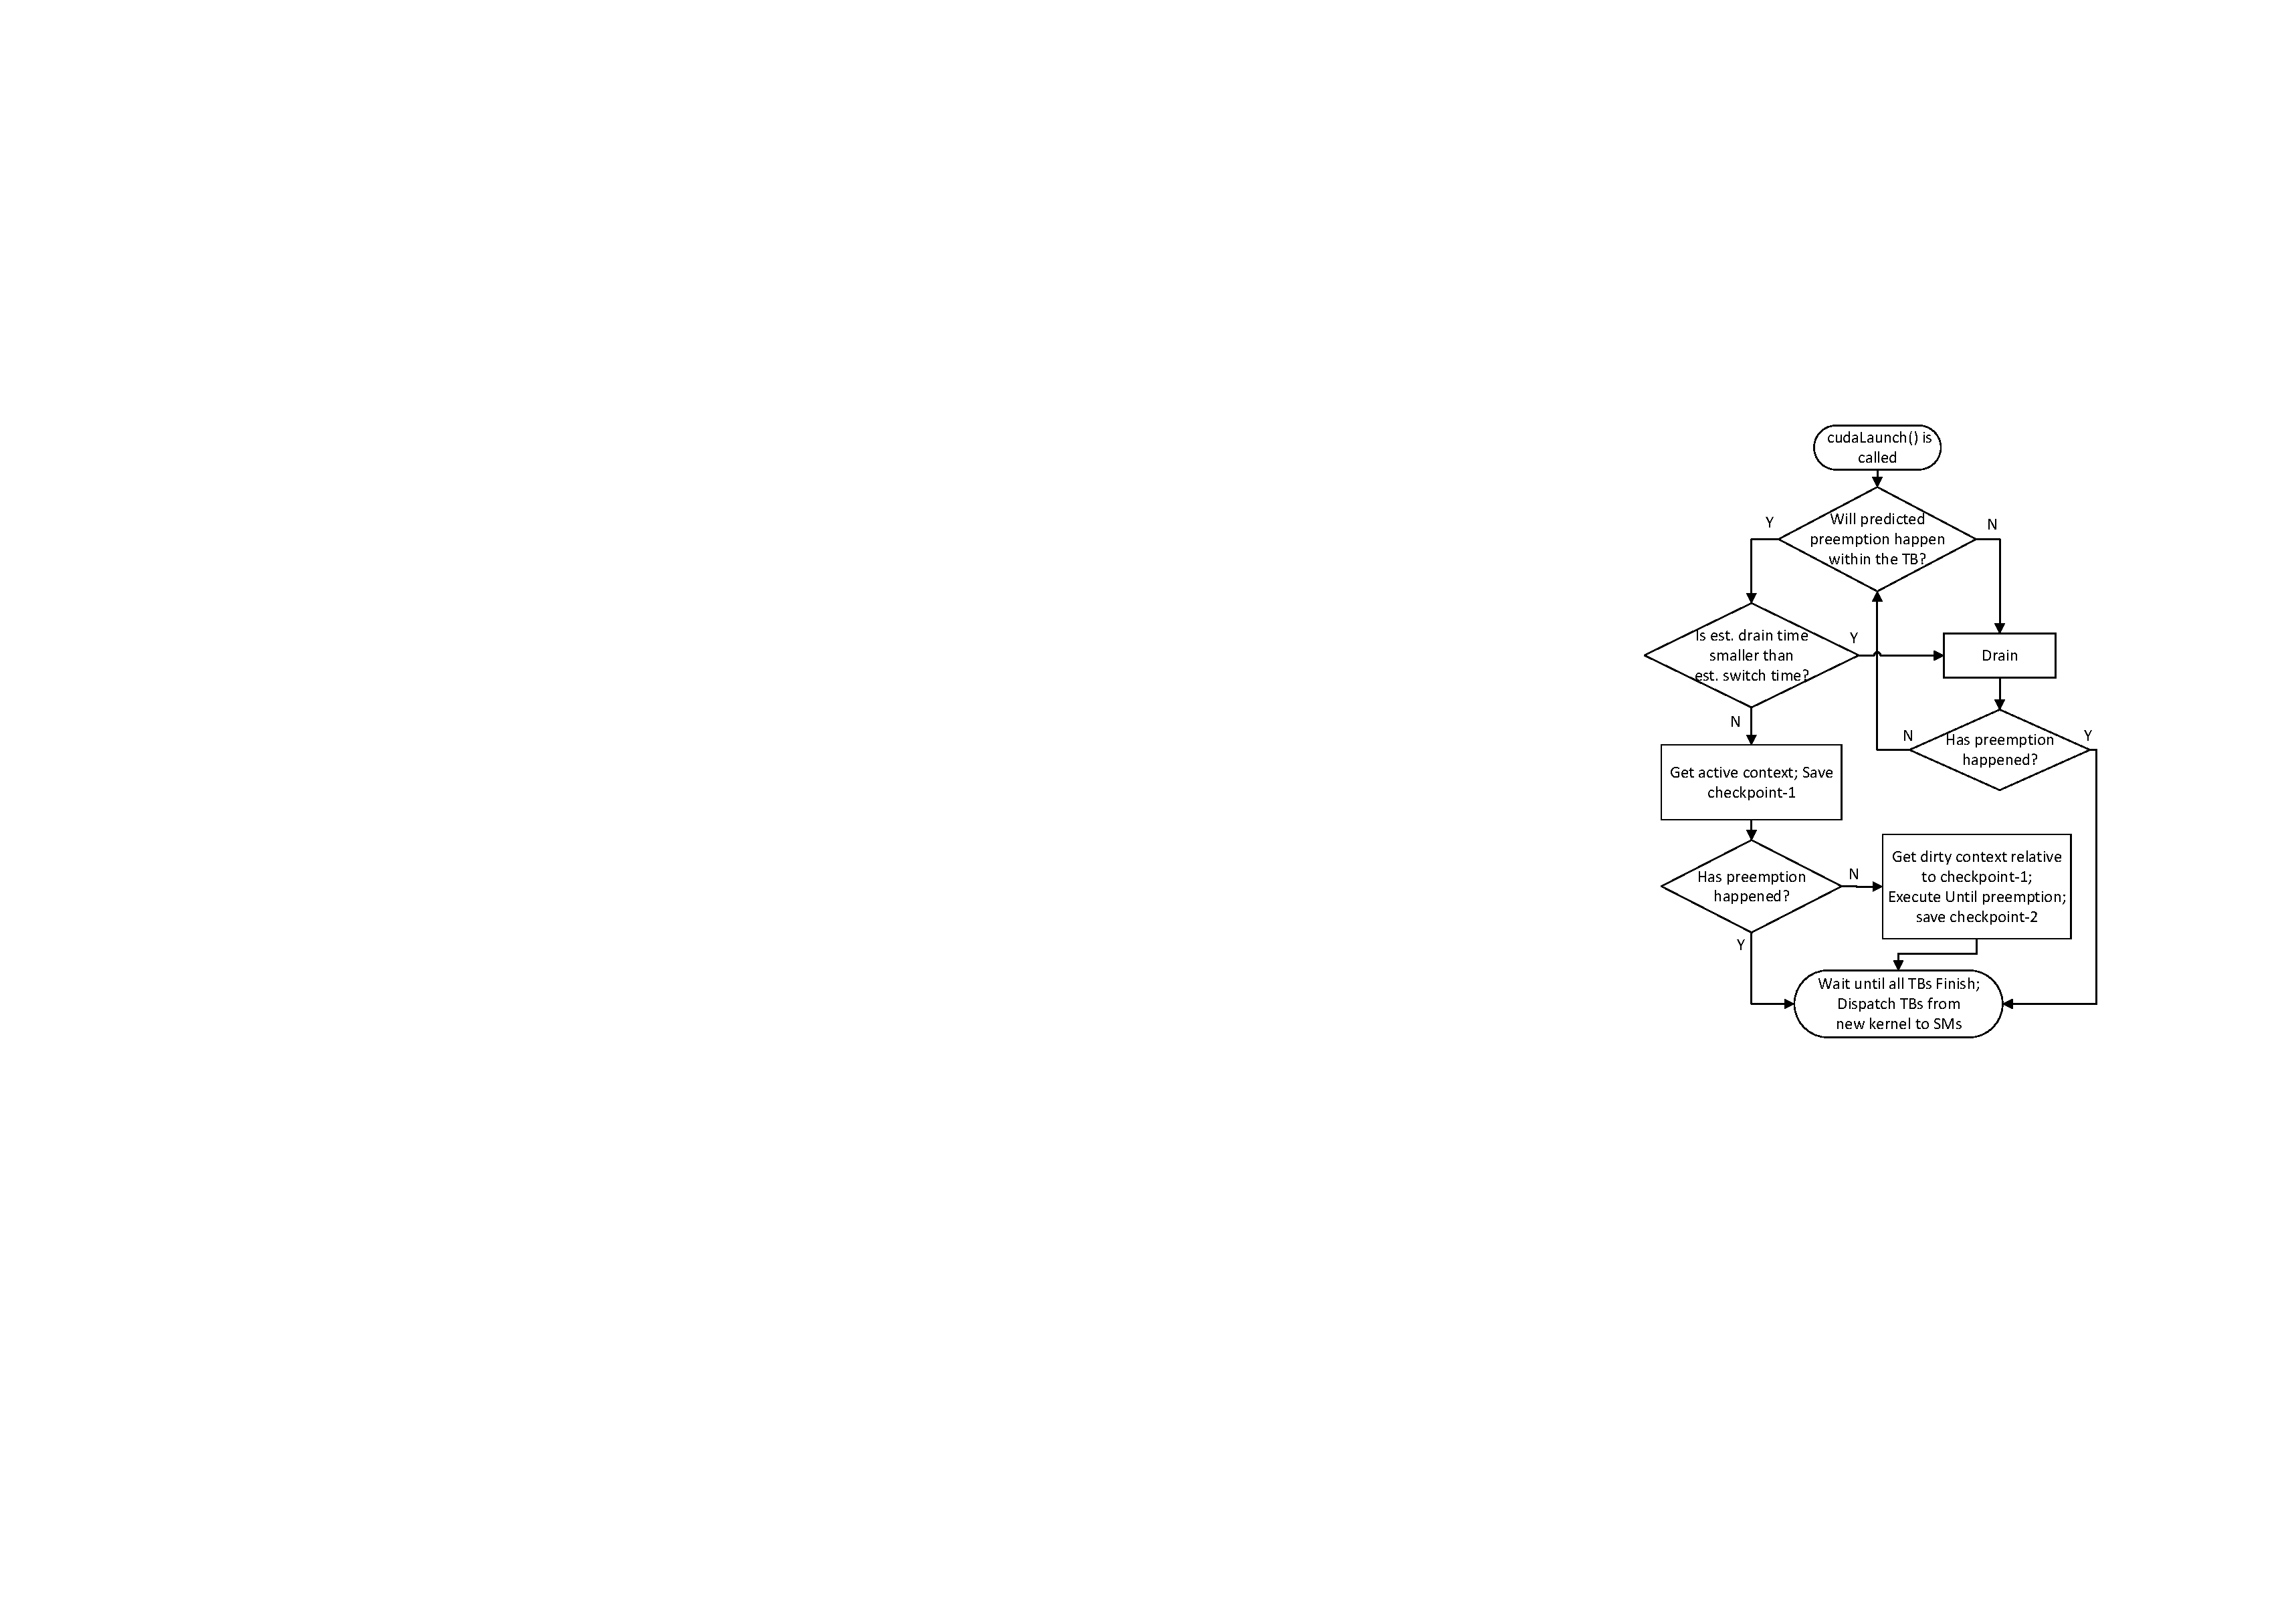
\includegraphics[width=.9\textwidth]{/Figs_PEP/design_flow}
  \caption{在线选择策略}
  \label{fig:design_flow}
\end{figure}

本章设计了一种动态在线选择机制来处理这些可能性。
图~\ref{fig:design_flow}阐述了在线选择方法。
当抢占内核函数的cudaLaunch被调用,PEP比较预测的内核函数启动时间与估计的当前线程块的剩余执行时间。
如果线程块的估计排空时间比上下文切换时间长,则定义该内核函数为长内核函数。
(a)和(b)均处理的是长内核函数,收集活跃的上下文,并用检查点备份的方法存储到全局内存。
对于其他的情况,内核函数预计的抢占点将不会在当前执行的线程块的生命周期中发生,
因此先排空执行当前的线程块。
当前内核函数分派新的线程块后再重新做时间的预测和估计。
如果新的线程块可以及时排空执行完毕,才发生抢占,则可以考虑(c)的情况。
否则,我们考虑(d)的方案。
这是(b)的另一种情况,而(e)是(a)的另一种情况。



\subsection{硬件开销}
为了实现PEP,GPU需要增加新的控制逻辑,主要为了实现以下部件:
(1)时间预测和估计单元,主要包括一些用来收集数据的计数器和比较器来完成选择;
(2)脏位,每个寄存器都需要一位,对于NVIDIA GTX 980 GPU~\upcite{nvidia980s},总计每个GPU核心需要8KB;
(3)分析计数器,该计数器用来收集线程块的执行时间。
综上,PEP最主要的硬件开销来源是脏位的存储开销。


\section{实验}
\label{sec:pepexperiment}

\subsection{实验方法}
本章在最新版本的GPGPU-Sim~\upcite{gpgpu-sim}中实现了PEP,以及Chimera。
系统配置信息总结在了表~\ref{table:configuration}。
配置中256KB寄存器和96KB的共享内存反映了当前GPU系统结构中较大的上下文。
默认情况下,GPGPU-Sim仅模拟PTX指令,是一种不限制寄存器使用数量的汇编伪指令集,并无法直接在硬件中执行,而SASS才是在硬件上执行的原生指令集。
因此,我们采用一种能够和SASS一一对应的PTXPlus指令集进行模拟,能够准确的模拟寄存器脏位。

\begin{table}[t]
  \centering
  \begin{tabular}{|l|l|}  
    \hline
    配置 & NVIDIA Geforce GTX 980\\
    \hline
    \hline
    GPU核心数量 & 16\\
    \hline
    SIMD宽度 & 32\\
    \hline
    SIMT核心时钟频率 & 1216MHz\\
    \hline
    存储时钟频率 & 7GHz\\
    \hline
    访存控制器数目 & 4 \\
    \hline
    调度策略 & 4个warp调度器采用Loose-Round-Robin策略\\
    \hline
    寄存器大小 & 256KB\\
    \hline
    共享内存大小 & 96KB\\
    \hline
    每个GPU核心的线程块数目最大值 & 32\\
    \hline
  \end{tabular}
  \caption{GPGPU-Sim参数配置}
 \label{table:configuration}
\end{table}


为了比较,本章实现了多个不同版本的Chimera和PEP:原生的Chimera、采用脏上下文的Chimera、原生的PEP以及采用了本地上下文备份的PEP。
我们测试了许多内核函数,这些内核函数来自于多个测试集的GPGPU应用程序,包括NVIDIA Computing SDK~\upcite{nvidia2013computing}、Parboil~\upcite{parboil}、Rodinia~\upcite{rodinia}和Darknet~\upcite{redmon2016yolo9000}等。
对于Chimera,我们设置了不同的内核函数延迟要求。
我们观察到上下文切换的平均时间总是小于20.9$\mu$s,因此将延迟要求分别设置为5$\mu$s、10$\mu$s和15$\mu$s。
对于PEP,我们设置了多个抢占内核函数的启动时间,预测的内核函数启动时间以及不同的抢占时机。
PEP的相关参数我们将在稍后讨论。
本章在实验中分别比较了这些不同设计的抢占延迟、上下文大小、以及抢占开销。

因为GPGPU-sim不模拟从cudaLaunch API调用到内核函数在GPU真正开始的时机,
我们设计了自己的实验方法。
我们采用NVIDIA profiler~\upcite{nvidiaprof}来收集分析内核函数启动所需要的时间,这个时间如表~\ref{table:time}所示,从3$\mu$s到33$\mu$s不等。
我们之后设置抢占内核函数的启动时间分别为5$\mu$s、15$\mu$s、25$\mu$s或35$\mu$s不等。
我们还设置了预测的内核函数启动时间为20$\mu$s或30$\mu$s。
此外,抢占可以发生在被抢占内核函数执行的任何阶段,因此我们设置了不同的抢占cudaLaunch调用的时机。
为了实验的目的,本章将抢占内核函数的cudaLaunch的调用时间分别设置在被抢占内核函数的平均线程块执行阶段的25\%、50\%和75\%。
因此,实验中每个应用程序将跑24次,取所有可能性的值的平均值。
下面的实验结果均为以各参数运行一次后的平均值。


\subsection{实验结果}

\subsubsection{策略选择分布}
如图~\ref{fig:distribution}所示,我们收集了每个应用程序采用实时策略选择后所有线程块的策略分布。
对于线程块运行时间长于100$\mu$s(表~\ref{table:time}所示)的应用程序,所有的线程块均采用了两次检查点备份的抢占方法。
相对地,所有选择排空执行所有线程块的都是小内核函数,即平均线程块执行时间较短。
对于LBM,线程块的平均执行时间为30.1$\mu$s,而平均上下文切换时间为20.9$\mu$s。
他们的排空执行时间和上下文切换时间相差不大。
这种相近性使得多种策略选择的出现,一些线程块需要被排空执行,而另一部分线程块则需要检查点备份技术,这都取决于被抢占的线程块的执行阶段。
在单次检查点备份的情况中,由于省去了增量检查点备份,节省了开销并降低了延迟。

\begin{figure}[htbp] % use float package if you want it here
  \centering
  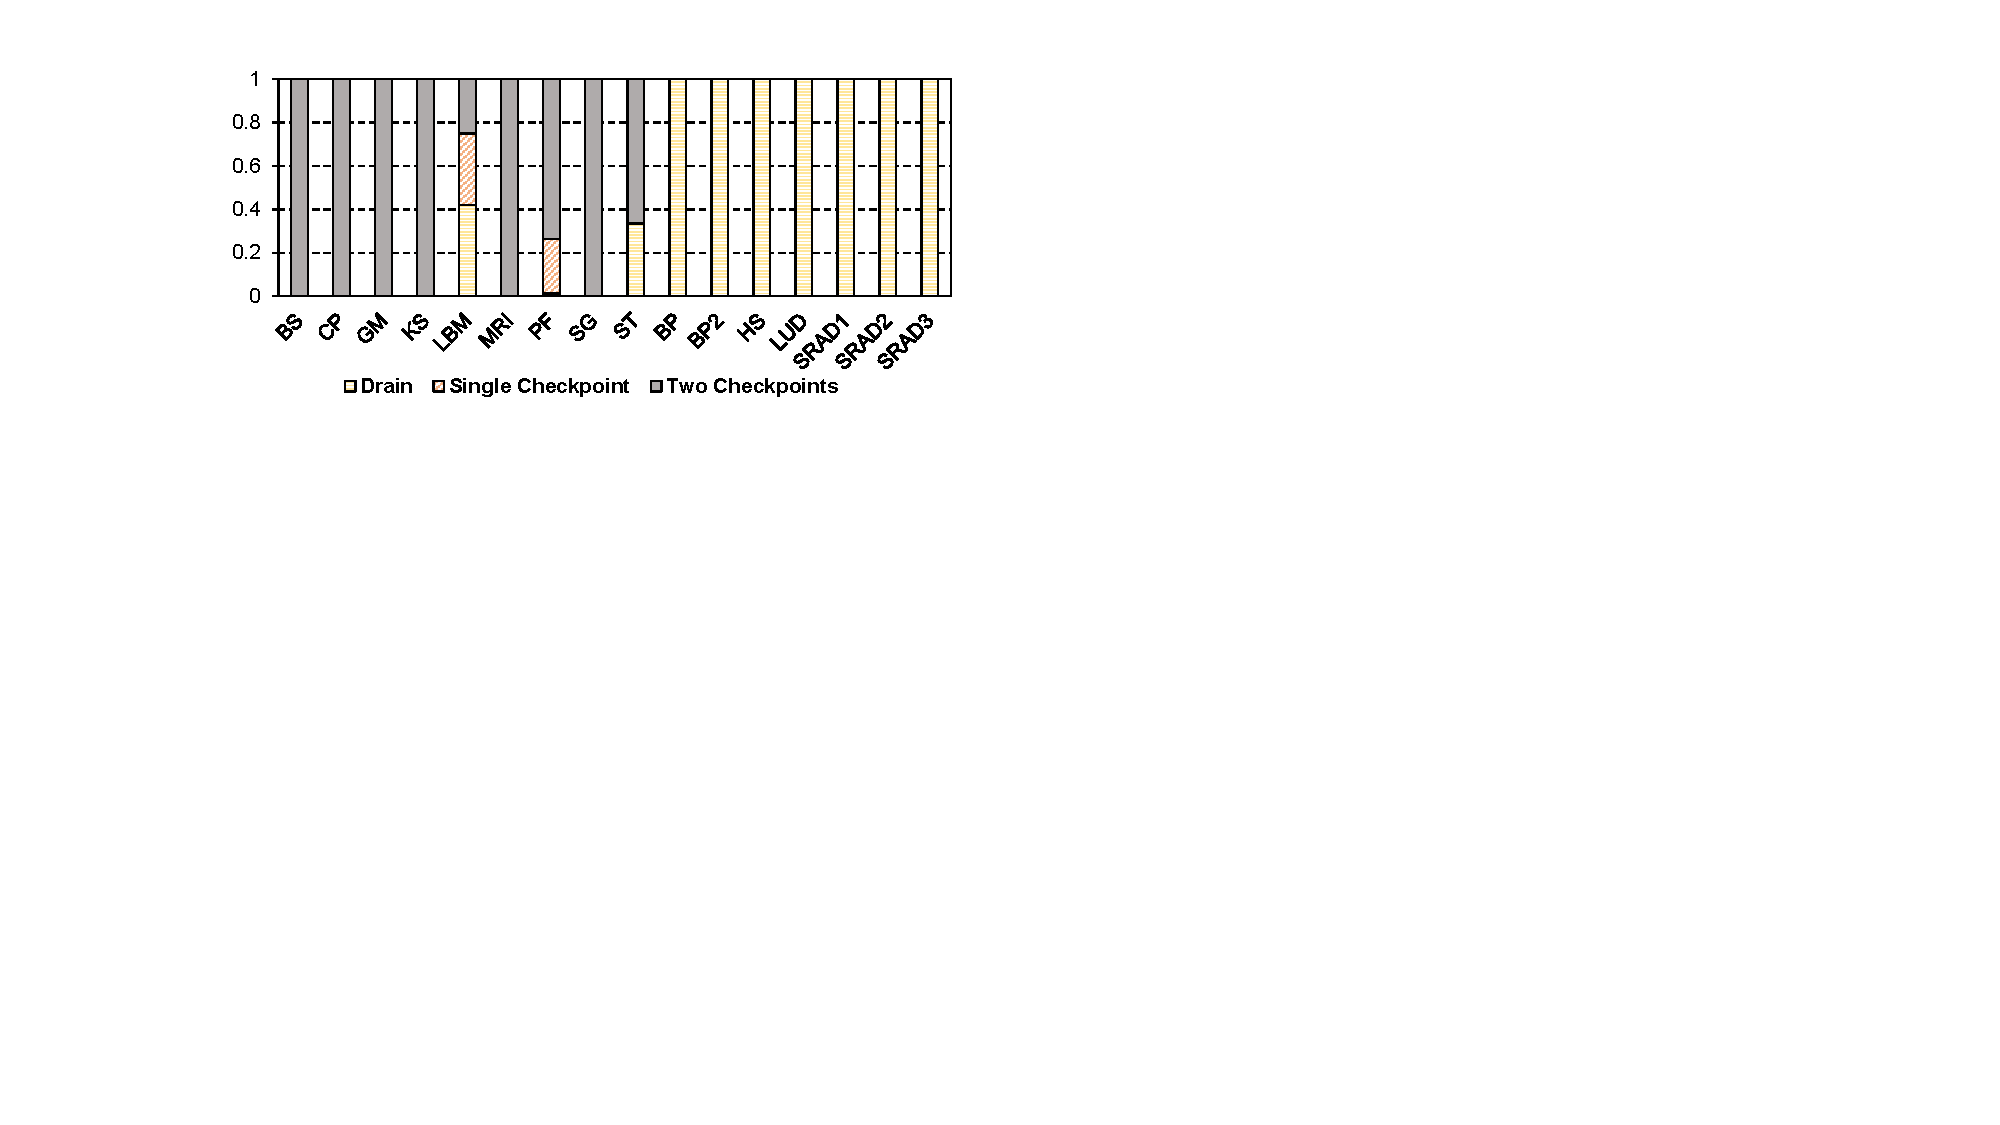
\includegraphics[width=.7\textwidth]{/Figs_PEP/distribution}
  \caption{抢占技术选择分布}
  \label{fig:distribution}
\end{figure}



由于对于大多数的内核函数,平均排空执行时间和平均上下文切换时间相差较大,我们大多数时候对所有的线程块选择一种抢占方法。
仅选择一种方法意味着排空执行的线程块的上下文切换的线程块之间没有带宽竞争。
因此,我们的延迟估计方法并不会收到访存冲突的影响。

\subsubsection{抢占延迟}

图~\ref{fig:preemptiontime}展示了抢占延迟,该延迟测量的是从抢占内核函数到达KMU开始到最后一个线程块的上下文被存储。
这也是内核函数等待池中抢占内核函数的真实等待时间。
我们观察到后面7个内核函数排空执行每个GPU核心中所有的线程块并达到了非常低的延迟。
这些应用程序的线程块执行时间也都相对较短。
虽然Chimera的时间估计方法并不准确,但Chimera选择的策略和PEP一样。
这是由于排空执行时间和上下文切换时间相差巨大,这并不要求非常高的精确度。
于是,所有四种方法在排空执行时延迟相同,平均排空执行时间为3.4$\mu$s。
但是,PEP和PEP+In-place分别将总平均抢占延迟从Chimera的8.9$\mu$s降低到4.5$\mu$s和3.6$\mu$s。
较短的抢占延迟使得内核函数能够满足更严格的延迟要求,也增加了多任务处理的可用性。

\begin{figure}[htbp] % use float package if you want it here
  \centering
  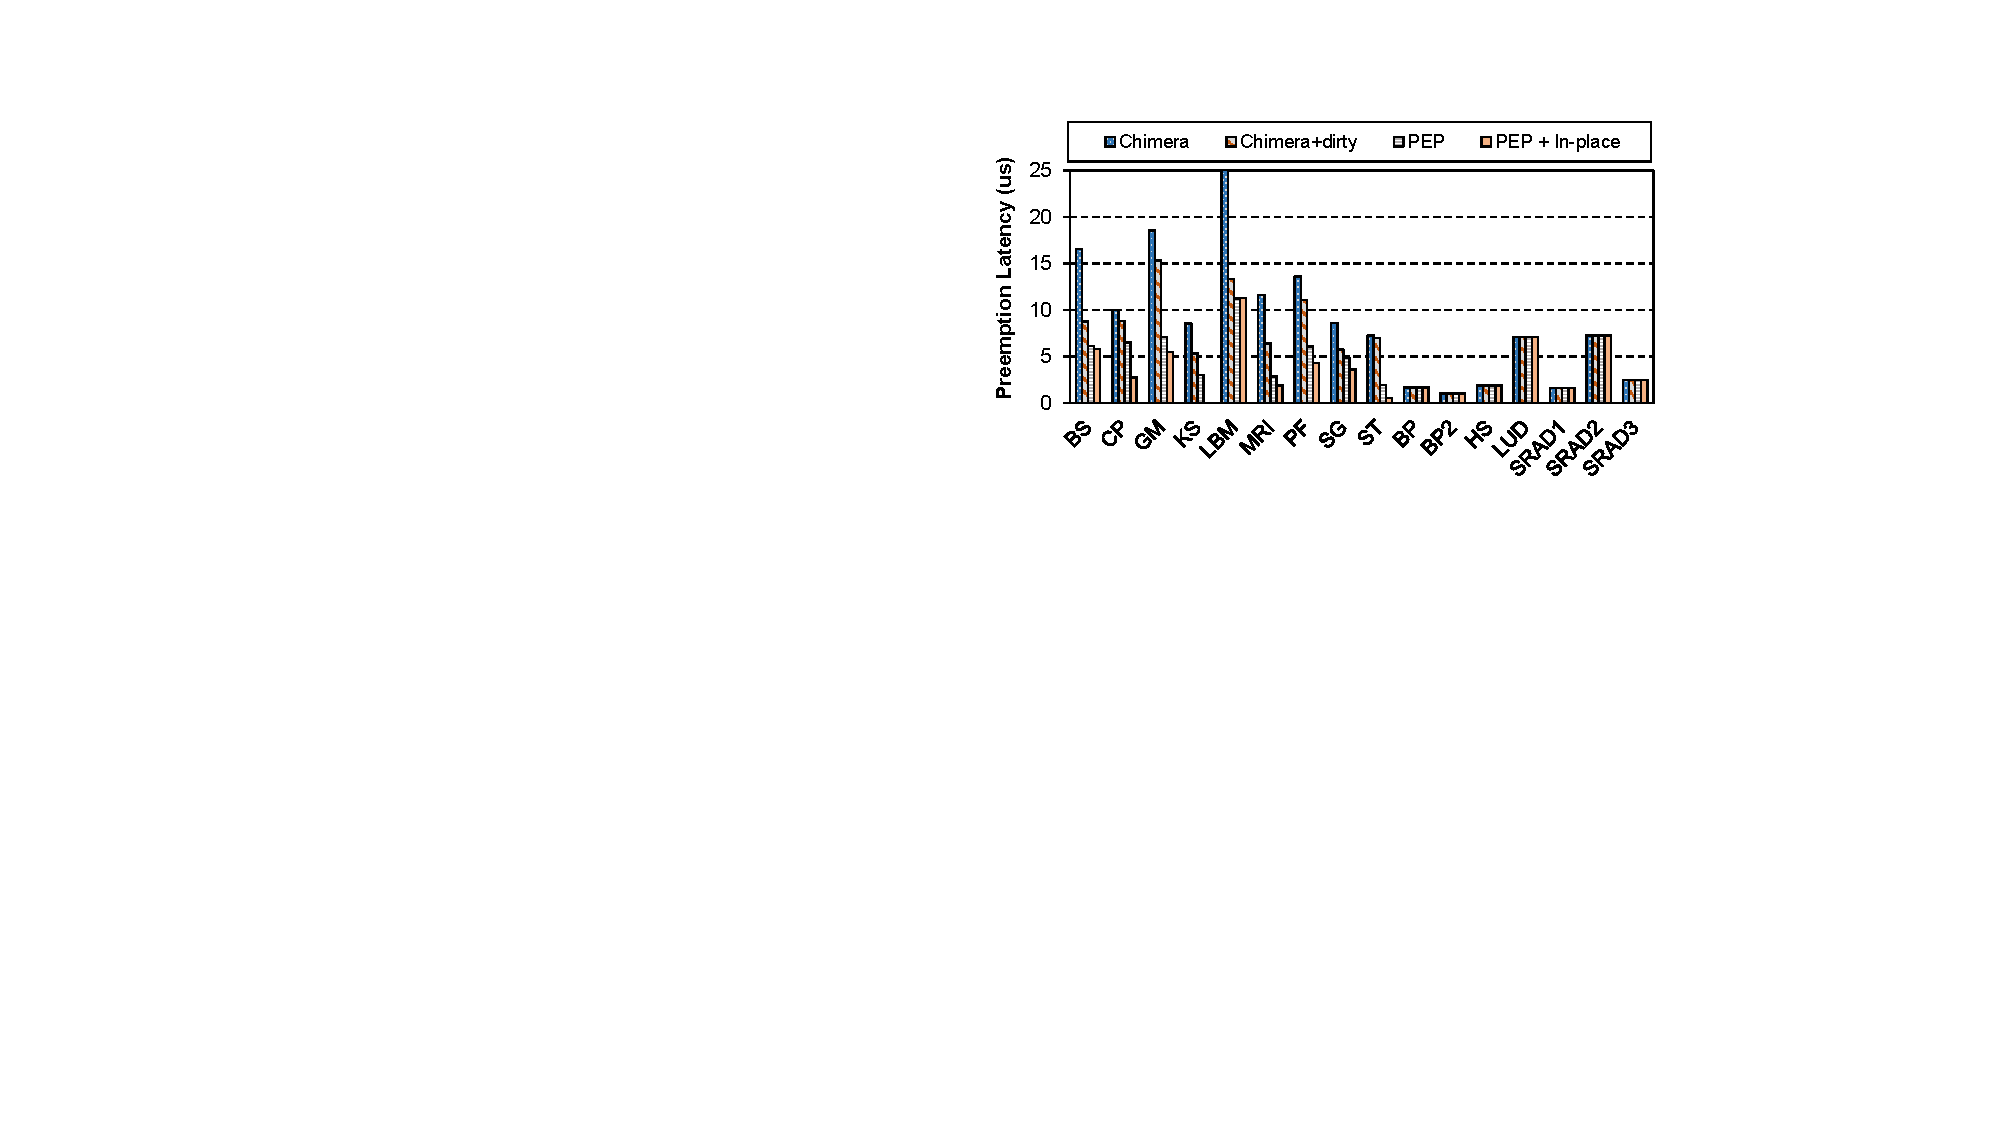
\includegraphics[width=.7\textwidth]{/Figs_PEP/preemptiontime}
  \caption{平均抢占延迟}
  \label{fig:preemptiontime}
\end{figure}


图~\ref{fig:normalized_preemptiontime}展示了上下文切换的抢占延迟。
前面的9个应用程序不会选择排空执行所有的线程块。
两个主要因素会影响他们的抢占延迟:流水线排空的时间和总的上下文大小。
这其中,上下文大小为关键因素。
与原生Chimera相比,脏上下文存储的Chimera能够降低31.8\%的抢占延迟,因为该方法减少了需要存储的上下文大小。
而与原生Chimera相比,PEP能够将平均抢占延迟降低了58.5\%,而采用了本地上下文存储后,PEP能进一步将抢占延迟降低70.3\%。
对于Kmeans(KS),PEP-In-place可以达到零抢占延迟,因为脏上下文的大小非常小,在增量检查点备份中可以完全存储于本地。

\begin{figure}[htbp] % use float package if you want it here
  \centering
  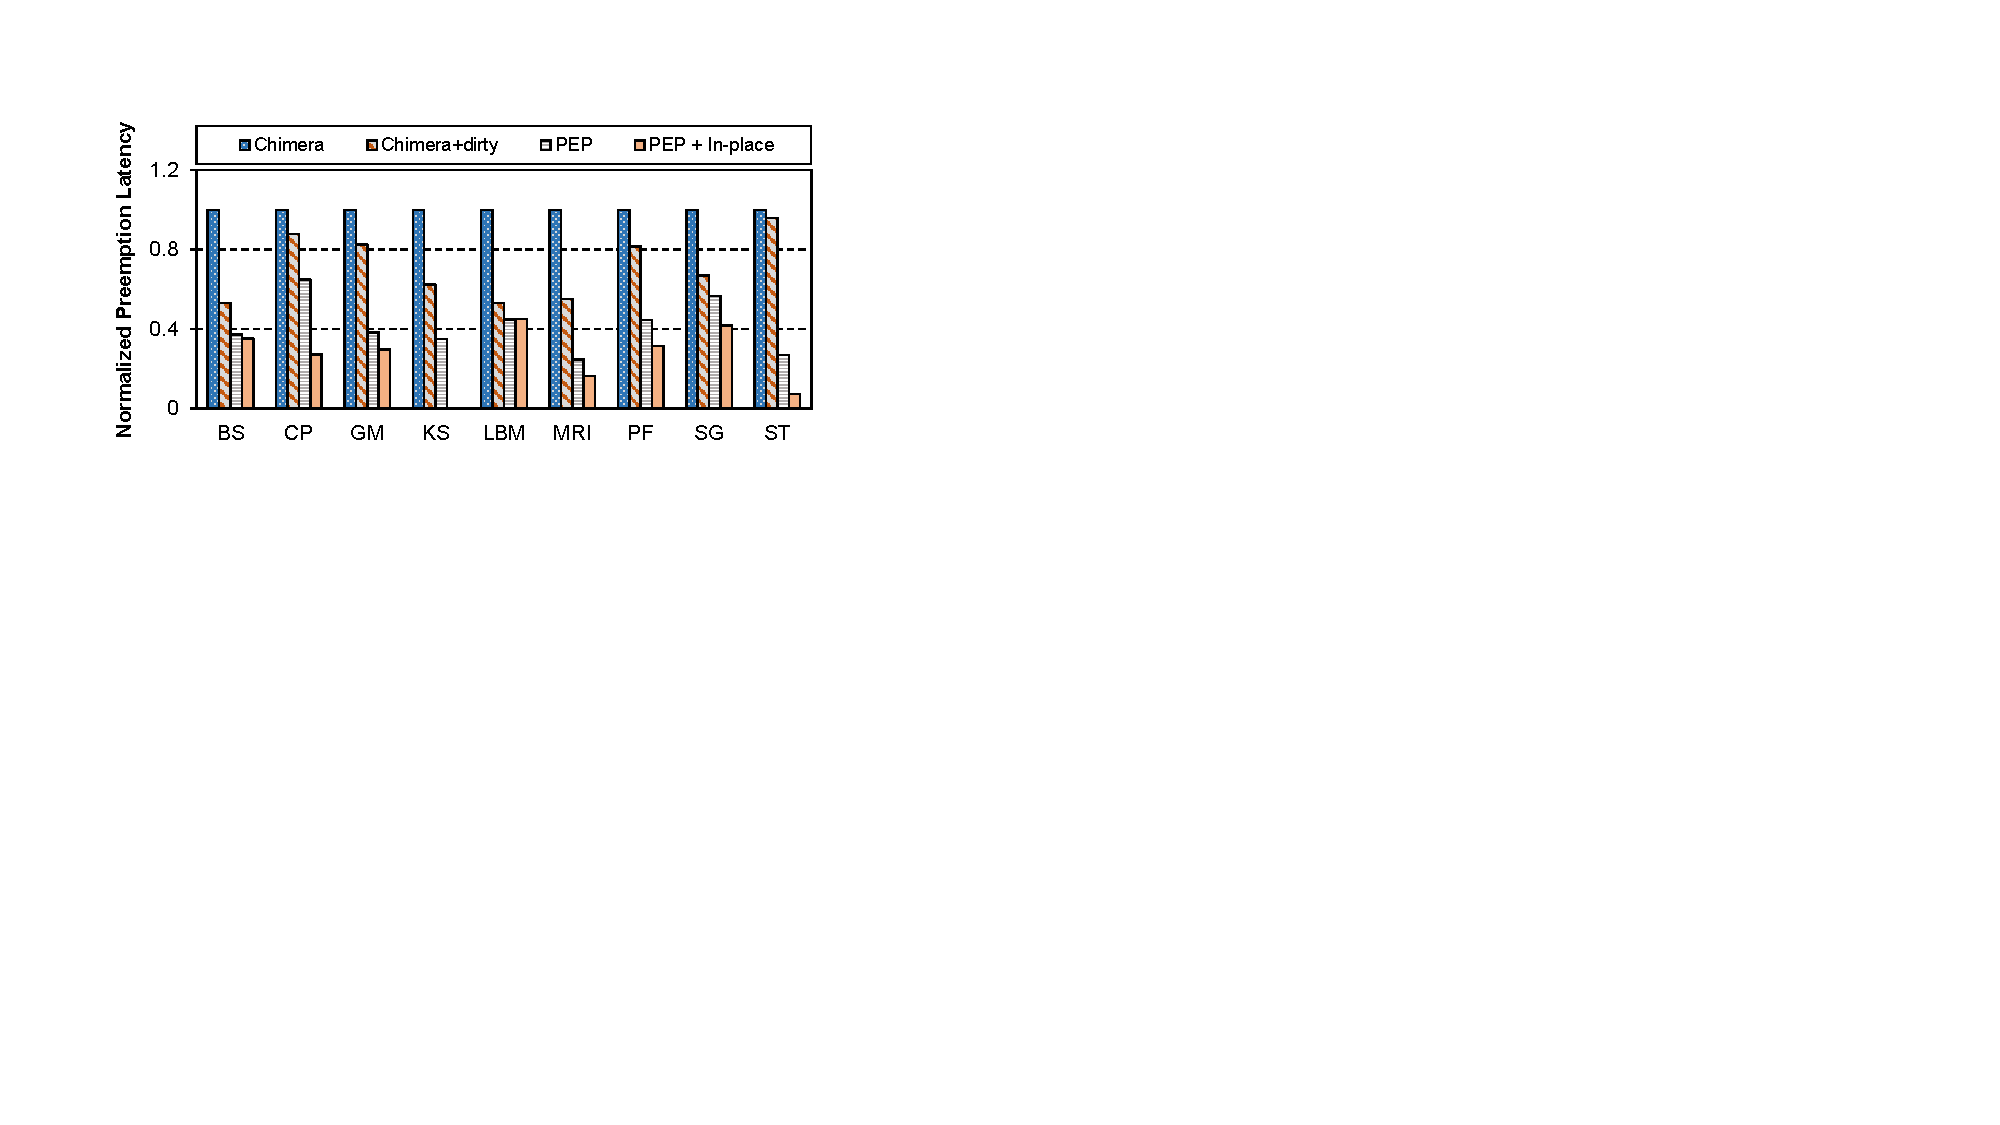
\includegraphics[width=.7\textwidth]{/Figs_PEP/normalized_preemptiontime}
  \caption{上下文切换应用程序的平均抢占延迟}
  \label{fig:normalized_preemptiontime}
\end{figure}

\subsubsection{上下文大小缩减}

在实验中的上下文,我们只考虑寄存器和共享内存。
共享内存位于片内,因此访存开销非常小。
程序员采用共享内存的目的是为了减少全局内存访问的开销,经常访问的数据将被放进共享内存。
因此,共享内存的脏位经常更新,开销较大。
我们仅将脏位应用于寄存器。大多数情况都将存储所有分配的共享内存。
在我们实验结果中,``上下文大小''指的是必须存储到全局内存的上下文。

图~\ref{fig:Contextsize1}比较了不同设计需要存储的上下文,只存储脏上下文,Chimera每个线程块的平均上下文大小可以被减少6KB,即平均总上下文大小的34.4\%。
因为PEP可能会存储检查点状态的上下文两次,PEP平均总上下文会比Chimera+dirty要大.
但是这几乎和原生Chimera一样。然而,PEP-in-place可以进一步降低16.2\%上下文大小。

\begin{figure}[htbp] % use float package if you want it here
  \centering
  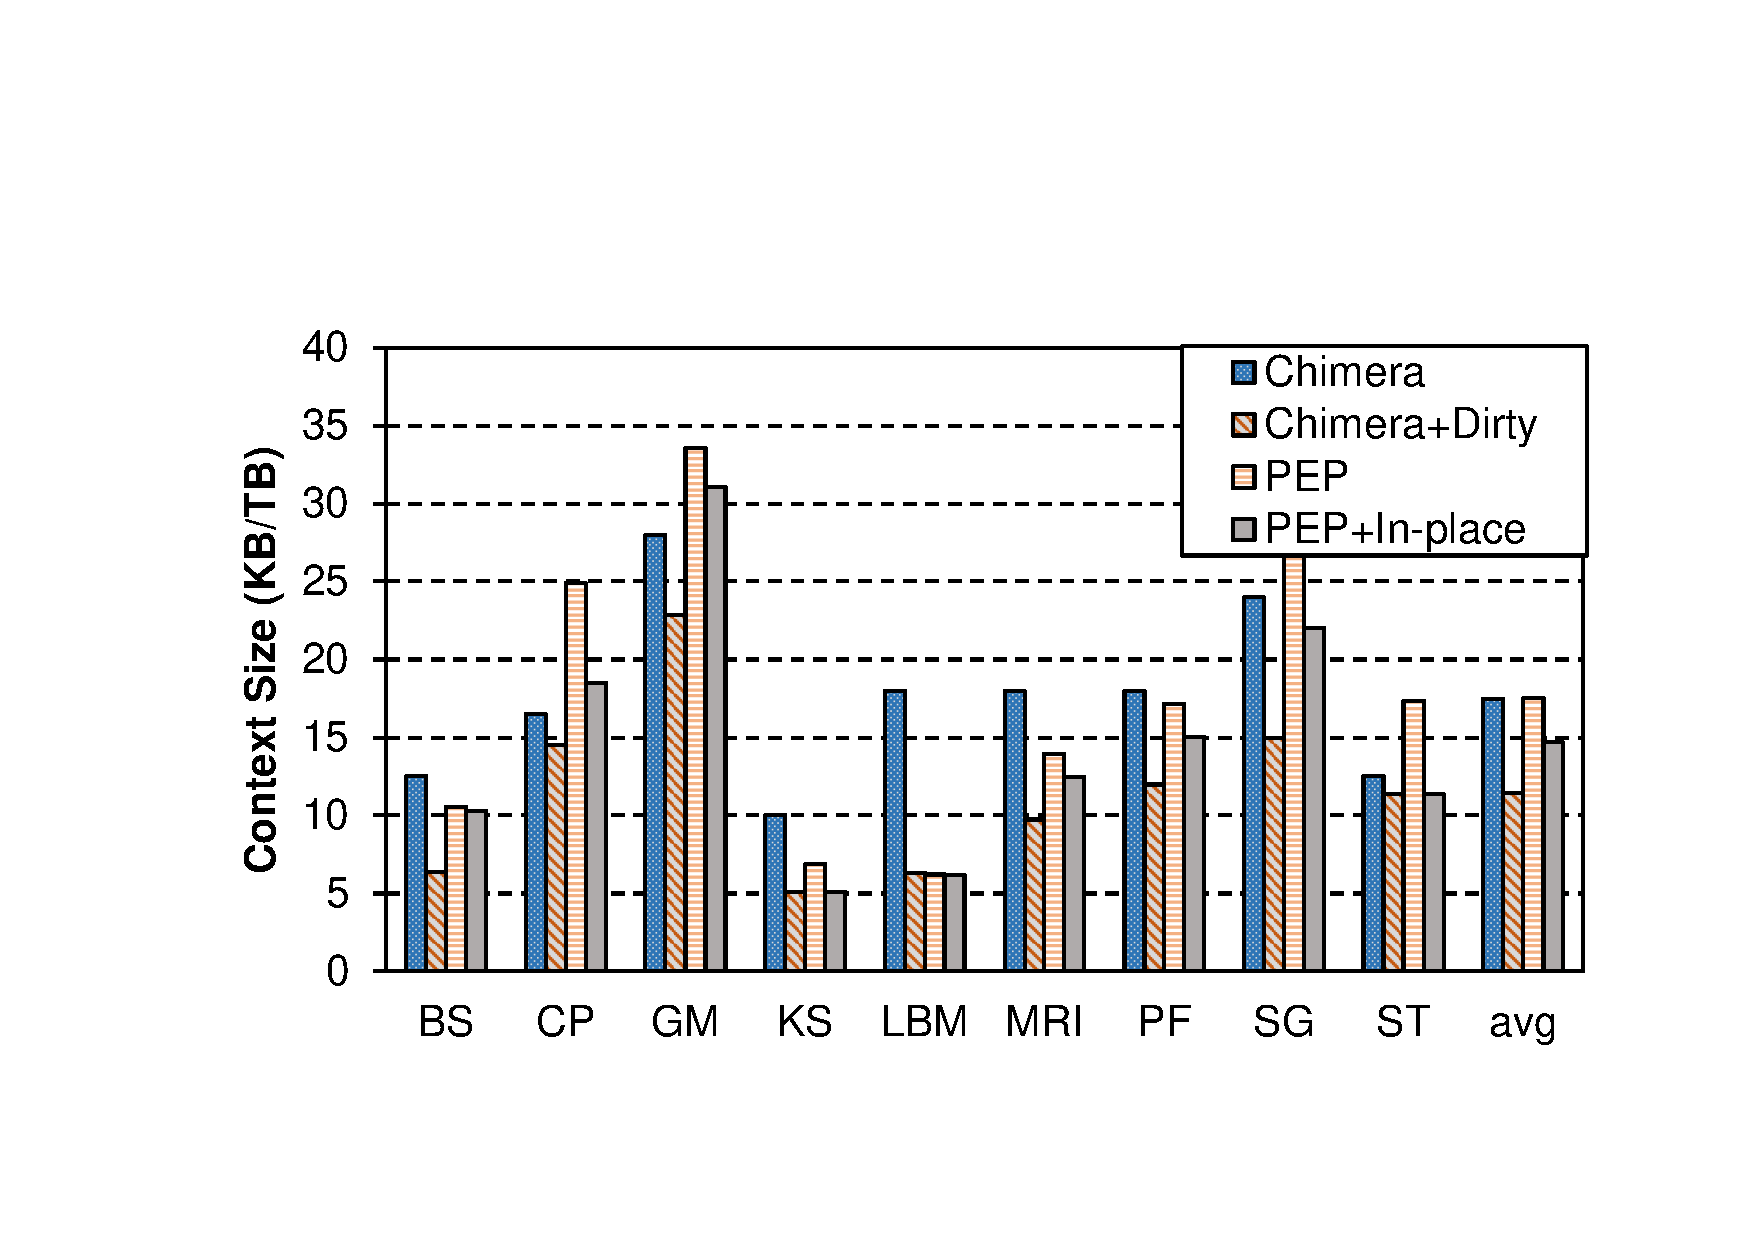
\includegraphics[width=.7\textwidth]{/Figs_PEP/Contextsize1}
  \caption{上下文大小比较}
  \label{fig:Contextsize1}
\end{figure}



图~\ref{fig:Contextsize3}和图~\ref{fig:Contextsize2}分别展示了PEP和PEP-in-place的上下文大小的细节。
对于选择上下文切换所有线程块的应用程序,总上下文大小为初始检查点备份和增量检查点备份的上下文大小之和。
实验结果显示增量上下文的大小平均只有基本上下文大小的56.1\%。
而本地上下文存储可以进一步降低增量检查点备份需存储的上下文。
图~\ref{fig:Contextsize2}的实验结果显示增量检查点备份的上下文大小平均为每个线程块3.34KB,是初始检查点备份的上下文的29.4\%。
我们可以看到两次检查点备份方法显著减少了上下文的大小。

\begin{figure}[htbp] % use float package if you want it here
  \centering
  \includegraphics[width=.7\textwidth]{/Figs_PEP/Contextsize3}
  \caption{需要备份到片外内存的每个线程块的上下文大小}
  \label{fig:Contextsize3}
\end{figure}

\begin{figure}[htbp] % use float package if you want it here
  \centering
  \includegraphics[width=.7\textwidth]{/Figs_PEP/Contextsize2}
  \caption{需要备份到片外内存的每个线程块的上下文大小(采用了本地上下文备份技术)}
  \label{fig:Contextsize2}
\end{figure}



\subsubsection{性能敏感分析}

在这一节,测试了带宽和可扩展性对性能的敏感性。

保持内存分区的数量和带宽,调整不同的GPU核心数量来分析他们对于PEP策略的抢占延迟的影响。
图~\ref{fig:sensitivity}展示了抢占延迟随着GPU核心数量的增加几乎线性增加,这是因为访存流量不断升高。
如图~\ref{fig:sensitivity}所示,32个GPU核心的平均抢占延迟是16个GPU核心的平均抢占延迟的2.58倍,这说明检查点策略对于存储带宽非常敏感。
因此,实验结果进一步说明所有的带宽都提供给上下文切换相比于将执行和上下文切换混合在一起,抢占性能更好。

\begin{figure}[htbp] % use float package if you want it here
  \centering
  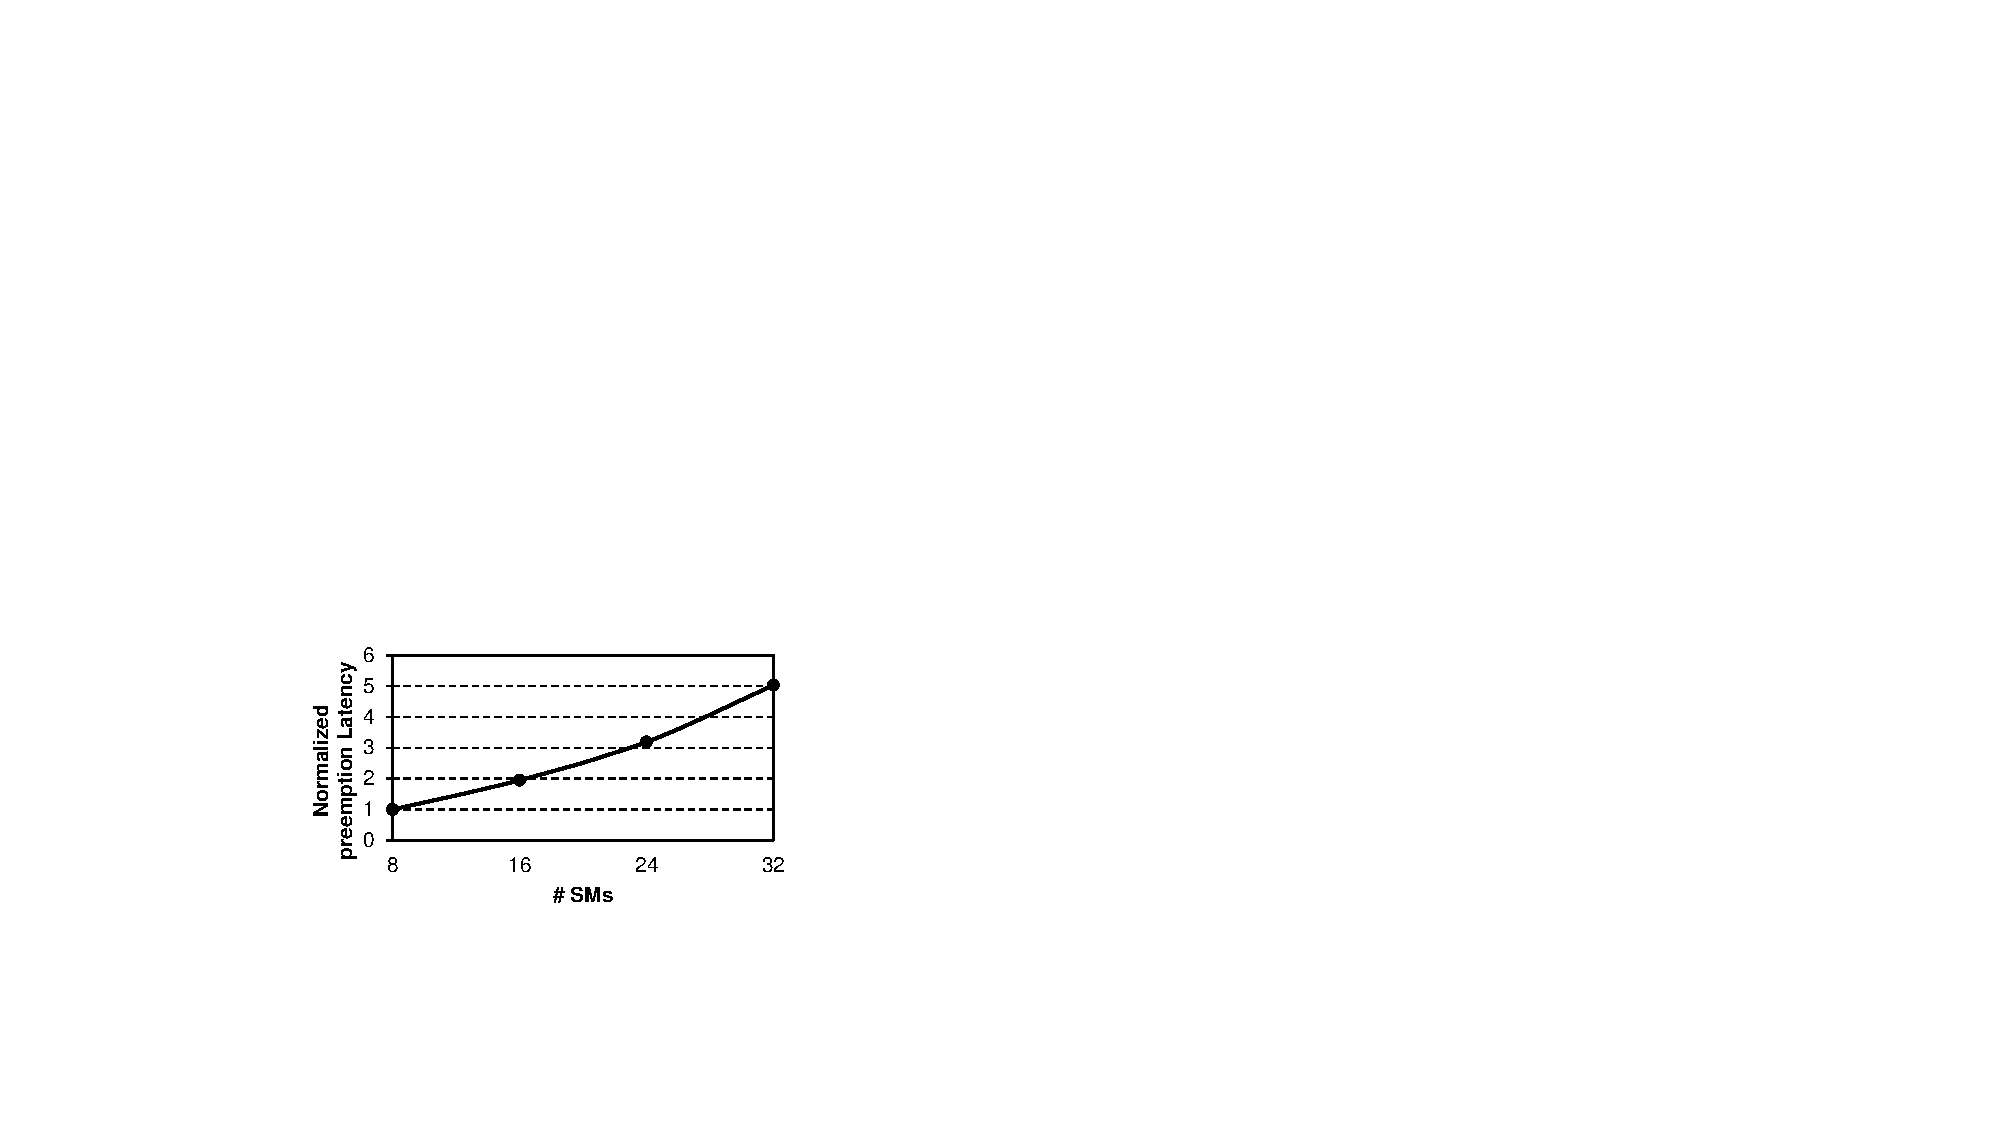
\includegraphics[width=.7\textwidth]{/Figs_PEP/sensitivity}
  \caption{GPU核心数量对于抢占技术的性能影响}
  \label{fig:sensitivity}
\end{figure}

\subsubsection{抢占开销分析}

本章所指的抢占开销是指由于抢占导致的程序执行的停滞时间。
抢占开销的实验结果如图~\ref{fig:overhead}所示。
当GPU核心在做上下文切换,切换的线程块必须停止取新指令和执行。
GPU核心停滞等待上下文备份和上下文恢复。
上下文备份和上下文恢复的唯一不同是上下文备份前排空流水线的延迟。
因此,我们只比较每个线程块的上下文切换延迟作为开销。
图~\ref{fig:overhead}显示初始检查点备份相比于Chimera开销降低了37.9\%。
PEP的开销和采用了脏上下文的Chimera的开销类似。
两次检查点备份的PEP开销仍然比Chimera降低了6.3\%。
当采用了本地上下文备份能够降低增量检查点备份的上下文大小,PEP的平均开销进一步降低了16.4\%。
一些应用程序相比于Chimera开销可能更高。
在这些情况中,寄存器的重用率不高,所以脏上下文的大小更大。
此外,采用了两次检查点备份,则更多的时间需要用来排空GPU核心的流水线。
但是,上下文的大小和上下文切换的开销是正相关的,一些应用程序向LBM和ST由于脏上下文大小较小,因此节省的开销大于50\%。

\begin{figure}[htbp] % use float package if you want it here
  \centering
  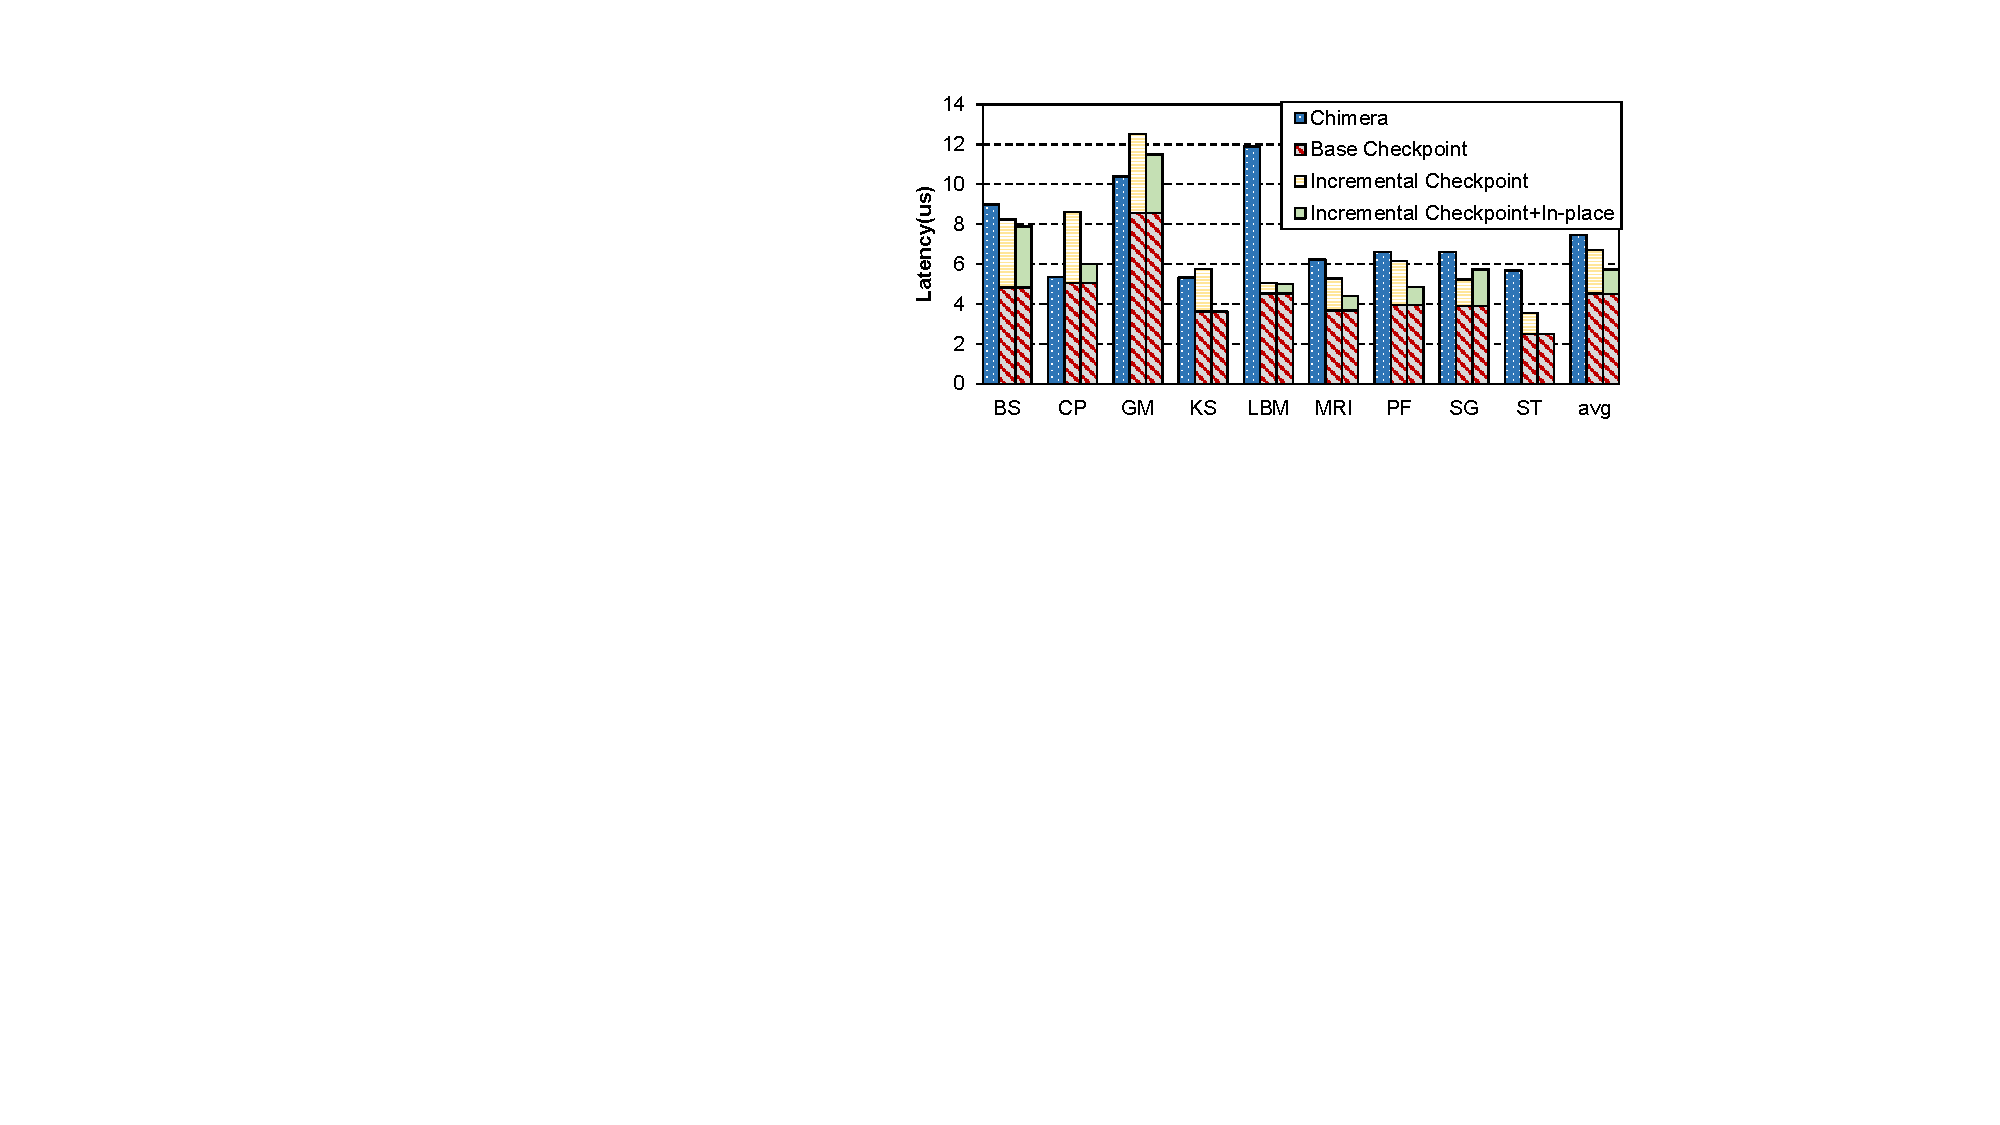
\includegraphics[width=.7\textwidth]{/Figs_PEP/overhead}
  \caption{上下文切换开销}
  \label{fig:overhead}
\end{figure}


\section{本章小结}
\label{sec:pepconclusion}
在本章,我们介绍了PEP,一种GPU动态主动的抢占机制。
只需要一个粗略的抢占内核函数启动时间的预测,就可以在抢占请求到来之前做好准备。
本章借鉴了容错中用到的检查点备份机制,允许我们缩短抢占延迟。
更重要的是检查点备份技术能够容忍不精确的预测。
为了预测抢占的发,我们利用了GPU驱动的内核函数启动的过程。
GPU驱动在收到CPU的内核函数启动的命令后会触发初始检查点备份。
这允许我们在真正的抢占请求到来时,只需要再备份相对于初始检查点备份变化的部分(增量)。
而GPU核心可以在两次检查点备份之间正常执行。
我们同时支持对小内核函数的GPU核心排空执行,还有本地上下文存储的功能来达到最小的抢占开销。
PEP主动检查点备份的抢占机制平均降低了58.6\%的抢占延迟和23.3\%的上下文切换开销。
平均抢占延迟也可以被降低到3.6$\mu$s,使得抢占应用程序能够满足更严格的延迟要求,更好地支持多任务。